\documentclass[twoside]{book}

% Packages required by doxygen
\usepackage{fixltx2e}
\usepackage{calc}
\usepackage{doxygen}
\usepackage[export]{adjustbox} % also loads graphicx
\usepackage{graphicx}
\usepackage[utf8]{inputenc}
\usepackage{makeidx}
\usepackage{multicol}
\usepackage{multirow}
\PassOptionsToPackage{warn}{textcomp}
\usepackage{textcomp}
\usepackage[nointegrals]{wasysym}
\usepackage[table]{xcolor}

% Font selection
\usepackage[T1]{fontenc}
\usepackage[scaled=.90]{helvet}
\usepackage{courier}
\usepackage{amssymb}
\usepackage{sectsty}
\renewcommand{\familydefault}{\sfdefault}
\allsectionsfont{%
  \fontseries{bc}\selectfont%
  \color{darkgray}%
}
\renewcommand{\DoxyLabelFont}{%
  \fontseries{bc}\selectfont%
  \color{darkgray}%
}
\newcommand{\+}{\discretionary{\mbox{\scriptsize$\hookleftarrow$}}{}{}}

% Page & text layout
\usepackage{geometry}
\geometry{%
  a4paper,%
  top=2.5cm,%
  bottom=2.5cm,%
  left=2.5cm,%
  right=2.5cm%
}
\tolerance=750
\hfuzz=15pt
\hbadness=750
\setlength{\emergencystretch}{15pt}
\setlength{\parindent}{0cm}
\setlength{\parskip}{3ex plus 2ex minus 2ex}
\makeatletter
\renewcommand{\paragraph}{%
  \@startsection{paragraph}{4}{0ex}{-1.0ex}{1.0ex}{%
    \normalfont\normalsize\bfseries\SS@parafont%
  }%
}
\renewcommand{\subparagraph}{%
  \@startsection{subparagraph}{5}{0ex}{-1.0ex}{1.0ex}{%
    \normalfont\normalsize\bfseries\SS@subparafont%
  }%
}
\makeatother

% Headers & footers
\usepackage{fancyhdr}
\pagestyle{fancyplain}
\fancyhead[LE]{\fancyplain{}{\bfseries\thepage}}
\fancyhead[CE]{\fancyplain{}{}}
\fancyhead[RE]{\fancyplain{}{\bfseries\leftmark}}
\fancyhead[LO]{\fancyplain{}{\bfseries\rightmark}}
\fancyhead[CO]{\fancyplain{}{}}
\fancyhead[RO]{\fancyplain{}{\bfseries\thepage}}
\fancyfoot[LE]{\fancyplain{}{}}
\fancyfoot[CE]{\fancyplain{}{}}
\fancyfoot[RE]{\fancyplain{}{\bfseries\scriptsize Generated by Doxygen }}
\fancyfoot[LO]{\fancyplain{}{\bfseries\scriptsize Generated by Doxygen }}
\fancyfoot[CO]{\fancyplain{}{}}
\fancyfoot[RO]{\fancyplain{}{}}
\renewcommand{\footrulewidth}{0.4pt}
\renewcommand{\chaptermark}[1]{%
  \markboth{#1}{}%
}
\renewcommand{\sectionmark}[1]{%
  \markright{\thesection\ #1}%
}

% Indices & bibliography
\usepackage{natbib}
\usepackage[titles]{tocloft}
\setcounter{tocdepth}{3}
\setcounter{secnumdepth}{5}
\makeindex

% Hyperlinks (required, but should be loaded last)
\usepackage{ifpdf}
\ifpdf
  \usepackage[pdftex,pagebackref=true]{hyperref}
\else
  \usepackage[ps2pdf,pagebackref=true]{hyperref}
\fi
\hypersetup{%
  colorlinks=true,%
  linkcolor=blue,%
  citecolor=blue,%
  unicode%
}

% Custom commands
\newcommand{\clearemptydoublepage}{%
  \newpage{\pagestyle{empty}\cleardoublepage}%
}

\usepackage{caption}
\captionsetup{labelsep=space,justification=centering,font={bf},singlelinecheck=off,skip=4pt,position=top}

%===== C O N T E N T S =====

\begin{document}

% Titlepage & ToC
\hypersetup{pageanchor=false,
             bookmarksnumbered=true,
             pdfencoding=unicode
            }
\pagenumbering{alph}
\begin{titlepage}
\vspace*{7cm}
\begin{center}%
{\Large M\+B\+T\+I-\/test \\[1ex]\large 1.\+0.\+0-\/alpha }\\
\vspace*{1cm}
{\large Generated by Doxygen 1.8.13}\\
\end{center}
\end{titlepage}
\clearemptydoublepage
\pagenumbering{roman}
\tableofcontents
\clearemptydoublepage
\pagenumbering{arabic}
\hypersetup{pageanchor=true}

%--- Begin generated contents ---
\chapter{Namespace Index}
\section{Namespace List}
Here is a list of all namespaces with brief descriptions\+:\begin{DoxyCompactList}
\item\contentsline{section}{\hyperlink{namespace_classes}{Classes} }{\pageref{namespace_classes}}{}
\item\contentsline{section}{\hyperlink{namespace_classes_1_1_preferences}{Classes\textbackslash{}\+Preferences} }{\pageref{namespace_classes_1_1_preferences}}{}
\item\contentsline{section}{\hyperlink{namespace_classes_1_1_test}{Classes\textbackslash{}\+Test} }{\pageref{namespace_classes_1_1_test}}{}
\item\contentsline{section}{\hyperlink{namespace_classes_1_1_types}{Classes\textbackslash{}\+Types} }{\pageref{namespace_classes_1_1_types}}{}
\end{DoxyCompactList}

\chapter{Hierarchical Index}
\section{Class Hierarchy}
This inheritance list is sorted roughly, but not completely, alphabetically\+:\begin{DoxyCompactList}
\item \contentsline{section}{Preference}{\pageref{class_classes_1_1_preferences_1_1_preference}}{}
\begin{DoxyCompactList}
\item \contentsline{section}{Decorator}{\pageref{class_classes_1_1_preferences_1_1_decorator}}{}
\begin{DoxyCompactList}
\item \contentsline{section}{Feeling}{\pageref{class_classes_1_1_preferences_1_1_feeling}}{}
\item \contentsline{section}{Intuition}{\pageref{class_classes_1_1_preferences_1_1_intuition}}{}
\item \contentsline{section}{Judging}{\pageref{class_classes_1_1_preferences_1_1_judging}}{}
\item \contentsline{section}{Perceiving}{\pageref{class_classes_1_1_preferences_1_1_perceiving}}{}
\item \contentsline{section}{Sensing}{\pageref{class_classes_1_1_preferences_1_1_sensing}}{}
\item \contentsline{section}{Thinking}{\pageref{class_classes_1_1_preferences_1_1_thinking}}{}
\end{DoxyCompactList}
\item \contentsline{section}{Extraversion}{\pageref{class_classes_1_1_preferences_1_1_extraversion}}{}
\item \contentsline{section}{Introversion}{\pageref{class_classes_1_1_preferences_1_1_introversion}}{}
\end{DoxyCompactList}
\item \contentsline{section}{Question}{\pageref{class_classes_1_1_test_1_1_question}}{}
\item \contentsline{section}{Set}{\pageref{class_classes_1_1_test_1_1_set}}{}
\item \contentsline{section}{Test}{\pageref{class_classes_1_1_test_1_1_test}}{}
\item \contentsline{section}{Type}{\pageref{class_classes_1_1_types_1_1_type}}{}
\end{DoxyCompactList}

\chapter{Data Structure Index}
\section{Data Structures}
Here are the data structures with brief descriptions\+:\begin{DoxyCompactList}
\item\contentsline{section}{\hyperlink{class_classes_1_1_preferences_1_1_decorator}{Decorator} }{\pageref{class_classes_1_1_preferences_1_1_decorator}}{}
\item\contentsline{section}{\hyperlink{class_classes_1_1_preferences_1_1_extraversion}{Extraversion} }{\pageref{class_classes_1_1_preferences_1_1_extraversion}}{}
\item\contentsline{section}{\hyperlink{class_classes_1_1_preferences_1_1_feeling}{Feeling} }{\pageref{class_classes_1_1_preferences_1_1_feeling}}{}
\item\contentsline{section}{\hyperlink{class_classes_1_1_preferences_1_1_introversion}{Introversion} }{\pageref{class_classes_1_1_preferences_1_1_introversion}}{}
\item\contentsline{section}{\hyperlink{class_classes_1_1_preferences_1_1_intuition}{Intuition} }{\pageref{class_classes_1_1_preferences_1_1_intuition}}{}
\item\contentsline{section}{\hyperlink{class_classes_1_1_preferences_1_1_judging}{Judging} }{\pageref{class_classes_1_1_preferences_1_1_judging}}{}
\item\contentsline{section}{\hyperlink{class_classes_1_1_preferences_1_1_perceiving}{Perceiving} }{\pageref{class_classes_1_1_preferences_1_1_perceiving}}{}
\item\contentsline{section}{\hyperlink{class_classes_1_1_preferences_1_1_preference}{Preference} }{\pageref{class_classes_1_1_preferences_1_1_preference}}{}
\item\contentsline{section}{\hyperlink{class_classes_1_1_test_1_1_question}{Question} }{\pageref{class_classes_1_1_test_1_1_question}}{}
\item\contentsline{section}{\hyperlink{class_classes_1_1_preferences_1_1_sensing}{Sensing} }{\pageref{class_classes_1_1_preferences_1_1_sensing}}{}
\item\contentsline{section}{\hyperlink{class_classes_1_1_test_1_1_set}{Set} }{\pageref{class_classes_1_1_test_1_1_set}}{}
\item\contentsline{section}{\hyperlink{class_classes_1_1_test_1_1_test}{Test} }{\pageref{class_classes_1_1_test_1_1_test}}{}
\item\contentsline{section}{\hyperlink{class_classes_1_1_preferences_1_1_thinking}{Thinking} }{\pageref{class_classes_1_1_preferences_1_1_thinking}}{}
\item\contentsline{section}{\hyperlink{class_classes_1_1_types_1_1_type}{Type} }{\pageref{class_classes_1_1_types_1_1_type}}{}
\end{DoxyCompactList}

\chapter{File Index}
\section{File List}
Here is a list of all files with brief descriptions\+:\begin{DoxyCompactList}
\item\contentsline{section}{E\+:/\+Server/\+Open\+Server/domains/localhost/\+M\+B\+T\+I-\/test/\hyperlink{index_8php}{index.\+php} }{\pageref{index_8php}}{}
\item\contentsline{section}{E\+:/\+Server/\+Open\+Server/domains/localhost/\+M\+B\+T\+I-\/test/\+Classes/\+Preferences/\hyperlink{_decorator_8php}{Decorator.\+php} }{\pageref{_decorator_8php}}{}
\item\contentsline{section}{E\+:/\+Server/\+Open\+Server/domains/localhost/\+M\+B\+T\+I-\/test/\+Classes/\+Preferences/\hyperlink{_extraversion_8php}{Extraversion.\+php} }{\pageref{_extraversion_8php}}{}
\item\contentsline{section}{E\+:/\+Server/\+Open\+Server/domains/localhost/\+M\+B\+T\+I-\/test/\+Classes/\+Preferences/\hyperlink{_feeling_8php}{Feeling.\+php} }{\pageref{_feeling_8php}}{}
\item\contentsline{section}{E\+:/\+Server/\+Open\+Server/domains/localhost/\+M\+B\+T\+I-\/test/\+Classes/\+Preferences/\hyperlink{_introversion_8php}{Introversion.\+php} }{\pageref{_introversion_8php}}{}
\item\contentsline{section}{E\+:/\+Server/\+Open\+Server/domains/localhost/\+M\+B\+T\+I-\/test/\+Classes/\+Preferences/\hyperlink{_intuition_8php}{Intuition.\+php} }{\pageref{_intuition_8php}}{}
\item\contentsline{section}{E\+:/\+Server/\+Open\+Server/domains/localhost/\+M\+B\+T\+I-\/test/\+Classes/\+Preferences/\hyperlink{_judging_8php}{Judging.\+php} }{\pageref{_judging_8php}}{}
\item\contentsline{section}{E\+:/\+Server/\+Open\+Server/domains/localhost/\+M\+B\+T\+I-\/test/\+Classes/\+Preferences/\hyperlink{_perceiving_8php}{Perceiving.\+php} }{\pageref{_perceiving_8php}}{}
\item\contentsline{section}{E\+:/\+Server/\+Open\+Server/domains/localhost/\+M\+B\+T\+I-\/test/\+Classes/\+Preferences/\hyperlink{_preference_8php}{Preference.\+php} }{\pageref{_preference_8php}}{}
\item\contentsline{section}{E\+:/\+Server/\+Open\+Server/domains/localhost/\+M\+B\+T\+I-\/test/\+Classes/\+Preferences/\hyperlink{_sensing_8php}{Sensing.\+php} }{\pageref{_sensing_8php}}{}
\item\contentsline{section}{E\+:/\+Server/\+Open\+Server/domains/localhost/\+M\+B\+T\+I-\/test/\+Classes/\+Preferences/\hyperlink{_thinking_8php}{Thinking.\+php} }{\pageref{_thinking_8php}}{}
\item\contentsline{section}{E\+:/\+Server/\+Open\+Server/domains/localhost/\+M\+B\+T\+I-\/test/\+Classes/\+Test/\hyperlink{_question_8php}{Question.\+php} }{\pageref{_question_8php}}{}
\item\contentsline{section}{E\+:/\+Server/\+Open\+Server/domains/localhost/\+M\+B\+T\+I-\/test/\+Classes/\+Test/\hyperlink{_set_8php}{Set.\+php} }{\pageref{_set_8php}}{}
\item\contentsline{section}{E\+:/\+Server/\+Open\+Server/domains/localhost/\+M\+B\+T\+I-\/test/\+Classes/\+Test/\hyperlink{_classes_2_test_2_test_8php}{Test.\+php} }{\pageref{_classes_2_test_2_test_8php}}{}
\item\contentsline{section}{E\+:/\+Server/\+Open\+Server/domains/localhost/\+M\+B\+T\+I-\/test/\+Classes/\+Types/\hyperlink{_type_8php}{Type.\+php} }{\pageref{_type_8php}}{}
\item\contentsline{section}{E\+:/\+Server/\+Open\+Server/domains/localhost/\+M\+B\+T\+I-\/test/modules/\hyperlink{modules_2_test_8php}{test.\+php} }{\pageref{modules_2_test_8php}}{}
\item\contentsline{section}{E\+:/\+Server/\+Open\+Server/domains/localhost/\+M\+B\+T\+I-\/test/modules/\hyperlink{types_8php}{types.\+php} }{\pageref{types_8php}}{}
\end{DoxyCompactList}

\chapter{Namespace Documentation}
\hypertarget{namespace_classes}{}\section{Classes Namespace Reference}
\label{namespace_classes}\index{Classes@{Classes}}
\subsection*{Namespaces}
\begin{DoxyCompactItemize}
\item 
 \hyperlink{namespace_classes_1_1_preferences}{Preferences}
\item 
 \hyperlink{namespace_classes_1_1_test}{Test}
\item 
 \hyperlink{namespace_classes_1_1_types}{Types}
\end{DoxyCompactItemize}

\hypertarget{namespace_classes_1_1_preferences}{}\section{Classes\textbackslash{}Preferences Namespace Reference}
\label{namespace_classes_1_1_preferences}\index{Classes\textbackslash{}\+Preferences@{Classes\textbackslash{}\+Preferences}}
\subsection*{Data Structures}
\begin{DoxyCompactItemize}
\item 
class \hyperlink{class_classes_1_1_preferences_1_1_decorator}{Decorator}
\item 
class \hyperlink{class_classes_1_1_preferences_1_1_extraversion}{Extraversion}
\item 
class \hyperlink{class_classes_1_1_preferences_1_1_feeling}{Feeling}
\item 
class \hyperlink{class_classes_1_1_preferences_1_1_introversion}{Introversion}
\item 
class \hyperlink{class_classes_1_1_preferences_1_1_intuition}{Intuition}
\item 
class \hyperlink{class_classes_1_1_preferences_1_1_judging}{Judging}
\item 
class \hyperlink{class_classes_1_1_preferences_1_1_perceiving}{Perceiving}
\item 
class \hyperlink{class_classes_1_1_preferences_1_1_preference}{Preference}
\item 
class \hyperlink{class_classes_1_1_preferences_1_1_sensing}{Sensing}
\item 
class \hyperlink{class_classes_1_1_preferences_1_1_thinking}{Thinking}
\end{DoxyCompactItemize}


\subsection{Detailed Description}
Created by Php\+Storm. User\+: A7ttim Date\+: 04.\+10.\+2017 Time\+: 15\+:34

Created by Php\+Storm. User\+: A7ttim Date\+: 04.\+10.\+2017 Time\+: 15\+:00

Created by Php\+Storm. User\+: A7ttim Date\+: 04.\+10.\+2017 Time\+: 19\+:48

Created by Php\+Storm. User\+: A7ttim Date\+: 04.\+10.\+2017 Time\+: 15\+:18

Created by Php\+Storm. User\+: A7ttim Date\+: 04.\+10.\+2017 Time\+: 15\+:33

Created by Php\+Storm. User\+: A7ttim Date\+: 04.\+10.\+2017 Time\+: 19\+:49

Created by Php\+Storm. User\+: A7ttim Date\+: 04.\+10.\+2017 Time\+: 19\+:50

Created by Php\+Storm. User\+: A7ttim Date\+: 04.\+10.\+2017 Time\+: 14\+:49

Created by Php\+Storm. User\+: A7ttim Date\+: 04.\+10.\+2017 Time\+: 19\+:47 
\hypertarget{namespace_classes_1_1_test}{}\section{Classes\textbackslash{}Test Namespace Reference}
\label{namespace_classes_1_1_test}\index{Classes\textbackslash{}\+Test@{Classes\textbackslash{}\+Test}}
\subsection*{Data Structures}
\begin{DoxyCompactItemize}
\item 
class \hyperlink{class_classes_1_1_test_1_1_question}{Question}
\item 
class \hyperlink{class_classes_1_1_test_1_1_set}{Set}
\item 
class \hyperlink{class_classes_1_1_test_1_1_test}{Test}
\end{DoxyCompactItemize}


\subsection{Detailed Description}
Created by Php\+Storm. User\+: A7ttim Date\+: 17.\+10.\+2017 Time\+: 16\+:56

Created by Php\+Storm. User\+: A7ttim Date\+: 17.\+10.\+2017 Time\+: 17\+:00

Created by Php\+Storm. User\+: A7ttim Date\+: 17.\+10.\+2017 Time\+: 17\+:49 
\hypertarget{namespace_classes_1_1_types}{}\section{Classes\textbackslash{}Types Namespace Reference}
\label{namespace_classes_1_1_types}\index{Classes\textbackslash{}\+Types@{Classes\textbackslash{}\+Types}}
\subsection*{Data Structures}
\begin{DoxyCompactItemize}
\item 
class \hyperlink{class_classes_1_1_types_1_1_type}{Type}
\end{DoxyCompactItemize}


\subsection{Detailed Description}
Created by Php\+Storm. User\+: A7ttim Date\+: 04.\+10.\+2017 Time\+: 23\+:37 
\chapter{Data Structure Documentation}
\hypertarget{class_classes_1_1_preferences_1_1_decorator}{}\section{Decorator Class Reference}
\label{class_classes_1_1_preferences_1_1_decorator}\index{Decorator@{Decorator}}
Inheritance diagram for Decorator\+:\begin{figure}[H]
\begin{center}
\leavevmode
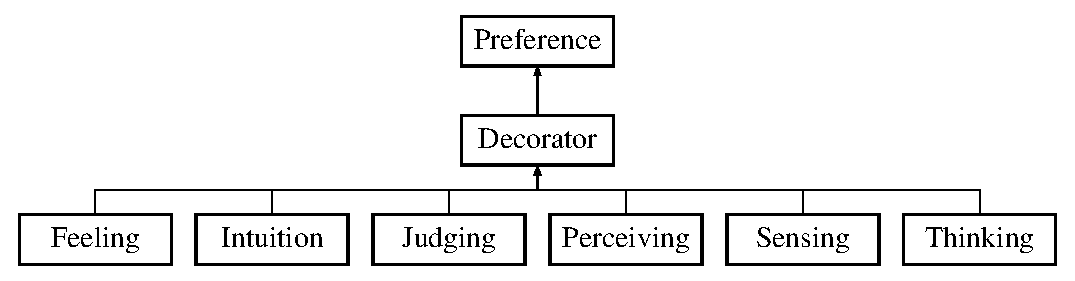
\includegraphics[height=3.000000cm]{class_classes_1_1_preferences_1_1_decorator}
\end{center}
\end{figure}
\subsection*{Public Member Functions}
\begin{DoxyCompactItemize}
\item 
\hyperlink{class_classes_1_1_preferences_1_1_decorator_a3b2b8d2271520af67fdf930580a59b12}{\+\_\+\+\_\+construct} (\hyperlink{class_classes_1_1_preferences_1_1_preference}{Preference} \$preference)
\item 
\hyperlink{class_classes_1_1_preferences_1_1_decorator_a2e7bb35c71bf1824456ceb944cb7a845}{get\+Description} ()
\item 
\hyperlink{class_classes_1_1_preferences_1_1_decorator_a830b5c75df72b32396701bc563fbe3c7}{get\+Type} ()
\end{DoxyCompactItemize}
\subsection*{Additional Inherited Members}


\subsection{Constructor \& Destructor Documentation}
\mbox{\Hypertarget{class_classes_1_1_preferences_1_1_decorator_a3b2b8d2271520af67fdf930580a59b12}\label{class_classes_1_1_preferences_1_1_decorator_a3b2b8d2271520af67fdf930580a59b12}} 
\index{Classes\+::\+Preferences\+::\+Decorator@{Classes\+::\+Preferences\+::\+Decorator}!\+\_\+\+\_\+construct@{\+\_\+\+\_\+construct}}
\index{\+\_\+\+\_\+construct@{\+\_\+\+\_\+construct}!Classes\+::\+Preferences\+::\+Decorator@{Classes\+::\+Preferences\+::\+Decorator}}
\subsubsection{\texorpdfstring{\+\_\+\+\_\+construct()}{\_\_construct()}}
{\footnotesize\ttfamily \+\_\+\+\_\+construct (\begin{DoxyParamCaption}\item[{\hyperlink{class_classes_1_1_preferences_1_1_preference}{Preference}}]{\$preference }\end{DoxyParamCaption})}



\subsection{Member Function Documentation}
\mbox{\Hypertarget{class_classes_1_1_preferences_1_1_decorator_a2e7bb35c71bf1824456ceb944cb7a845}\label{class_classes_1_1_preferences_1_1_decorator_a2e7bb35c71bf1824456ceb944cb7a845}} 
\index{Classes\+::\+Preferences\+::\+Decorator@{Classes\+::\+Preferences\+::\+Decorator}!get\+Description@{get\+Description}}
\index{get\+Description@{get\+Description}!Classes\+::\+Preferences\+::\+Decorator@{Classes\+::\+Preferences\+::\+Decorator}}
\subsubsection{\texorpdfstring{get\+Description()}{getDescription()}}
{\footnotesize\ttfamily get\+Description (\begin{DoxyParamCaption}{ }\end{DoxyParamCaption})}

\mbox{\Hypertarget{class_classes_1_1_preferences_1_1_decorator_a830b5c75df72b32396701bc563fbe3c7}\label{class_classes_1_1_preferences_1_1_decorator_a830b5c75df72b32396701bc563fbe3c7}} 
\index{Classes\+::\+Preferences\+::\+Decorator@{Classes\+::\+Preferences\+::\+Decorator}!get\+Type@{get\+Type}}
\index{get\+Type@{get\+Type}!Classes\+::\+Preferences\+::\+Decorator@{Classes\+::\+Preferences\+::\+Decorator}}
\subsubsection{\texorpdfstring{get\+Type()}{getType()}}
{\footnotesize\ttfamily get\+Type (\begin{DoxyParamCaption}{ }\end{DoxyParamCaption})}



The documentation for this class was generated from the following file\+:\begin{DoxyCompactItemize}
\item 
E\+:/\+Server/\+Open\+Server/domains/localhost/\+M\+B\+T\+I-\/test/\+Classes/\+Preferences/\hyperlink{_decorator_8php}{Decorator.\+php}\end{DoxyCompactItemize}

\hypertarget{class_classes_1_1_preferences_1_1_extraversion}{}\section{Extraversion Class Reference}
\label{class_classes_1_1_preferences_1_1_extraversion}\index{Extraversion@{Extraversion}}
Inheritance diagram for Extraversion\+:\begin{figure}[H]
\begin{center}
\leavevmode
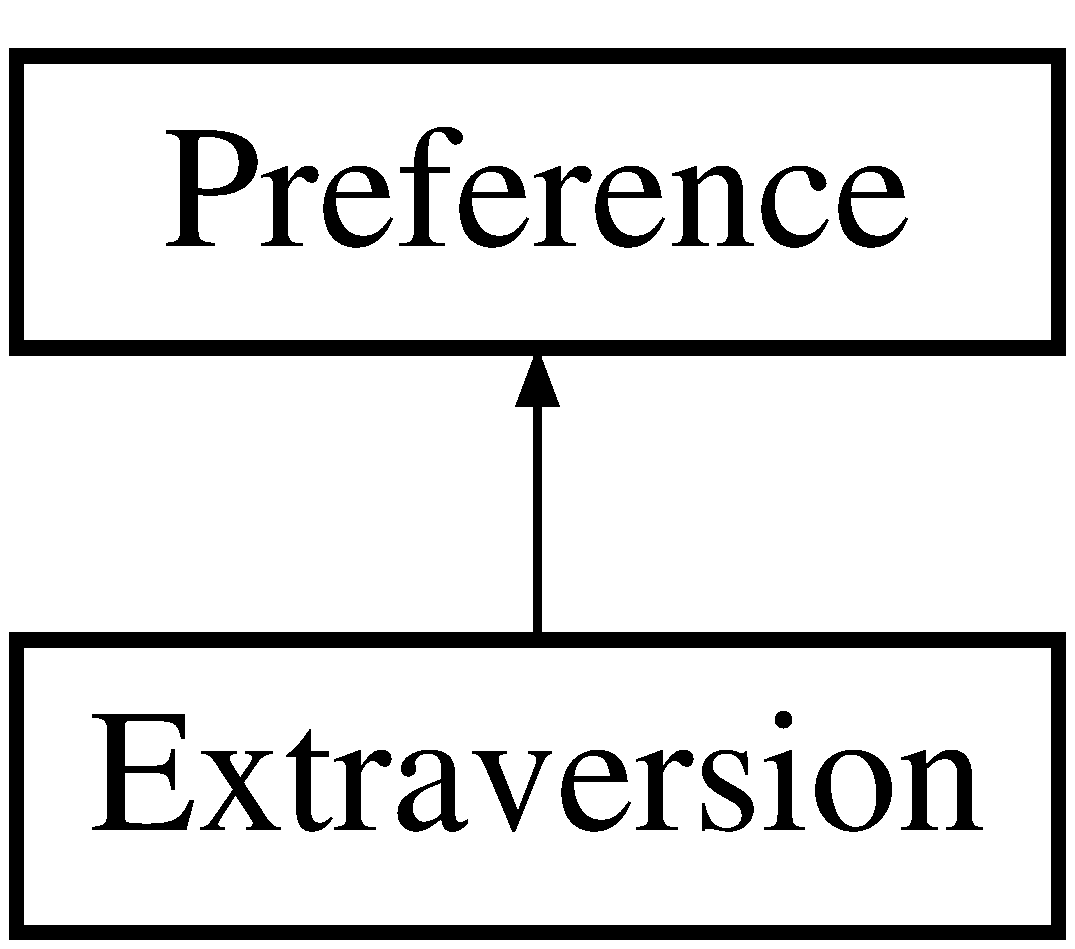
\includegraphics[height=2.000000cm]{class_classes_1_1_preferences_1_1_extraversion}
\end{center}
\end{figure}
\subsection*{Data Fields}
\begin{DoxyCompactItemize}
\item 
\hyperlink{class_classes_1_1_preferences_1_1_extraversion_aa04ae5f5f106925e87308c0520c0837a}{\$symbol} = \char`\"{}E\char`\"{}
\item 
\hyperlink{class_classes_1_1_preferences_1_1_extraversion_ab2fc40d43824ea3e1ce5d86dee0d763b}{\$name} = \char`\"{}Экстраверсия\char`\"{}
\item 
\hyperlink{class_classes_1_1_preferences_1_1_extraversion_a87b032cba06009e3467abf1c8018d960}{\$description} = \char`\"{}Ориентация сознания наружу, на объекты\char`\"{}
\end{DoxyCompactItemize}
\subsection*{Additional Inherited Members}


\subsection{Field Documentation}
\mbox{\Hypertarget{class_classes_1_1_preferences_1_1_extraversion_a87b032cba06009e3467abf1c8018d960}\label{class_classes_1_1_preferences_1_1_extraversion_a87b032cba06009e3467abf1c8018d960}} 
\index{Classes\+::\+Preferences\+::\+Extraversion@{Classes\+::\+Preferences\+::\+Extraversion}!\$description@{\$description}}
\index{\$description@{\$description}!Classes\+::\+Preferences\+::\+Extraversion@{Classes\+::\+Preferences\+::\+Extraversion}}
\subsubsection{\texorpdfstring{\$description}{$description}}
{\footnotesize\ttfamily \$description = \char`\"{}Ориентация сознания наружу, на объекты\char`\"{}}

\mbox{\Hypertarget{class_classes_1_1_preferences_1_1_extraversion_ab2fc40d43824ea3e1ce5d86dee0d763b}\label{class_classes_1_1_preferences_1_1_extraversion_ab2fc40d43824ea3e1ce5d86dee0d763b}} 
\index{Classes\+::\+Preferences\+::\+Extraversion@{Classes\+::\+Preferences\+::\+Extraversion}!\$name@{\$name}}
\index{\$name@{\$name}!Classes\+::\+Preferences\+::\+Extraversion@{Classes\+::\+Preferences\+::\+Extraversion}}
\subsubsection{\texorpdfstring{\$name}{$name}}
{\footnotesize\ttfamily \$name = \char`\"{}Экстраверсия\char`\"{}}

\mbox{\Hypertarget{class_classes_1_1_preferences_1_1_extraversion_aa04ae5f5f106925e87308c0520c0837a}\label{class_classes_1_1_preferences_1_1_extraversion_aa04ae5f5f106925e87308c0520c0837a}} 
\index{Classes\+::\+Preferences\+::\+Extraversion@{Classes\+::\+Preferences\+::\+Extraversion}!\$symbol@{\$symbol}}
\index{\$symbol@{\$symbol}!Classes\+::\+Preferences\+::\+Extraversion@{Classes\+::\+Preferences\+::\+Extraversion}}
\subsubsection{\texorpdfstring{\$symbol}{$symbol}}
{\footnotesize\ttfamily \$symbol = \char`\"{}E\char`\"{}}



The documentation for this class was generated from the following file\+:\begin{DoxyCompactItemize}
\item 
E\+:/\+Server/\+Open\+Server/domains/localhost/\+M\+B\+T\+I-\/test/\+Classes/\+Preferences/\hyperlink{_extraversion_8php}{Extraversion.\+php}\end{DoxyCompactItemize}

\hypertarget{class_classes_1_1_preferences_1_1_feeling}{}\section{Feeling Class Reference}
\label{class_classes_1_1_preferences_1_1_feeling}\index{Feeling@{Feeling}}
Inheritance diagram for Feeling\+:\begin{figure}[H]
\begin{center}
\leavevmode
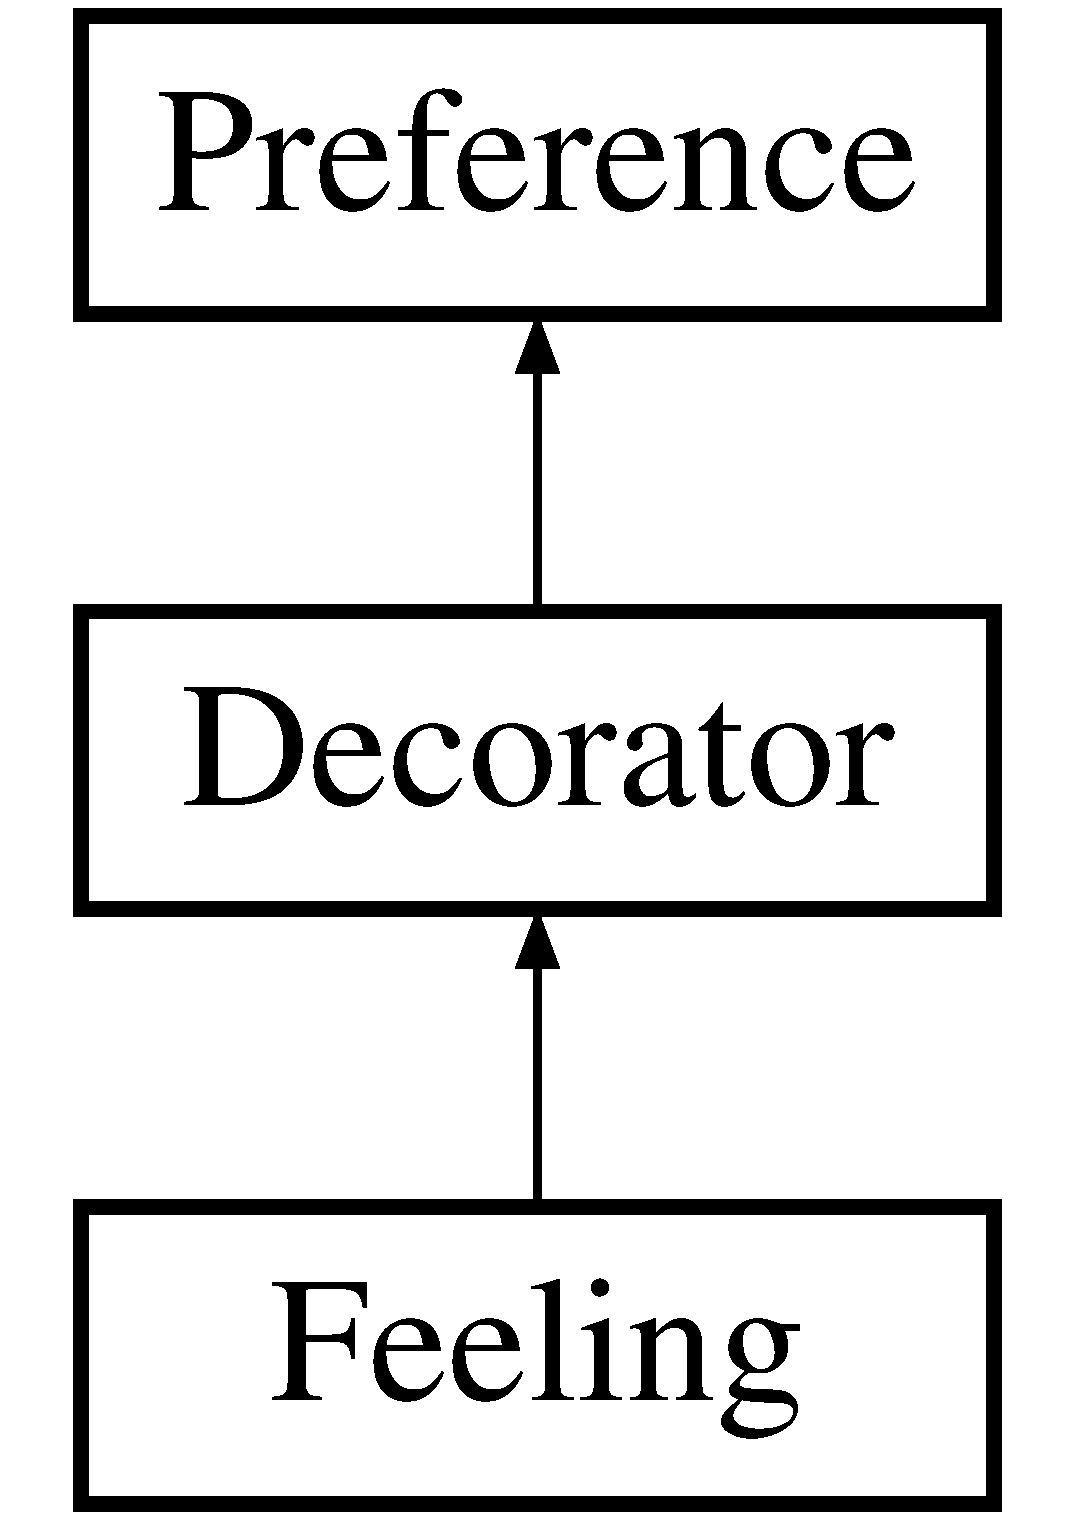
\includegraphics[height=3.000000cm]{class_classes_1_1_preferences_1_1_feeling}
\end{center}
\end{figure}
\subsection*{Data Fields}
\begin{DoxyCompactItemize}
\item 
\hyperlink{class_classes_1_1_preferences_1_1_feeling_aa04ae5f5f106925e87308c0520c0837a}{\$symbol} = \char`\"{}F\char`\"{}
\item 
\hyperlink{class_classes_1_1_preferences_1_1_feeling_ab2fc40d43824ea3e1ce5d86dee0d763b}{\$name} = \char`\"{}Чувство\char`\"{}
\item 
\hyperlink{class_classes_1_1_preferences_1_1_feeling_a87b032cba06009e3467abf1c8018d960}{\$description} = \char`\"{}Принятие решений на эмоциональной основе\char`\"{}
\end{DoxyCompactItemize}
\subsection*{Additional Inherited Members}


\subsection{Field Documentation}
\mbox{\Hypertarget{class_classes_1_1_preferences_1_1_feeling_a87b032cba06009e3467abf1c8018d960}\label{class_classes_1_1_preferences_1_1_feeling_a87b032cba06009e3467abf1c8018d960}} 
\index{Classes\+::\+Preferences\+::\+Feeling@{Classes\+::\+Preferences\+::\+Feeling}!\$description@{\$description}}
\index{\$description@{\$description}!Classes\+::\+Preferences\+::\+Feeling@{Classes\+::\+Preferences\+::\+Feeling}}
\subsubsection{\texorpdfstring{\$description}{$description}}
{\footnotesize\ttfamily \$description = \char`\"{}Принятие решений на эмоциональной основе\char`\"{}}

\mbox{\Hypertarget{class_classes_1_1_preferences_1_1_feeling_ab2fc40d43824ea3e1ce5d86dee0d763b}\label{class_classes_1_1_preferences_1_1_feeling_ab2fc40d43824ea3e1ce5d86dee0d763b}} 
\index{Classes\+::\+Preferences\+::\+Feeling@{Classes\+::\+Preferences\+::\+Feeling}!\$name@{\$name}}
\index{\$name@{\$name}!Classes\+::\+Preferences\+::\+Feeling@{Classes\+::\+Preferences\+::\+Feeling}}
\subsubsection{\texorpdfstring{\$name}{$name}}
{\footnotesize\ttfamily \$name = \char`\"{}Чувство\char`\"{}}

\mbox{\Hypertarget{class_classes_1_1_preferences_1_1_feeling_aa04ae5f5f106925e87308c0520c0837a}\label{class_classes_1_1_preferences_1_1_feeling_aa04ae5f5f106925e87308c0520c0837a}} 
\index{Classes\+::\+Preferences\+::\+Feeling@{Classes\+::\+Preferences\+::\+Feeling}!\$symbol@{\$symbol}}
\index{\$symbol@{\$symbol}!Classes\+::\+Preferences\+::\+Feeling@{Classes\+::\+Preferences\+::\+Feeling}}
\subsubsection{\texorpdfstring{\$symbol}{$symbol}}
{\footnotesize\ttfamily \$symbol = \char`\"{}F\char`\"{}}



The documentation for this class was generated from the following file\+:\begin{DoxyCompactItemize}
\item 
E\+:/\+Server/\+Open\+Server/domains/localhost/\+M\+B\+T\+I-\/test/\+Classes/\+Preferences/\hyperlink{_feeling_8php}{Feeling.\+php}\end{DoxyCompactItemize}

\hypertarget{class_classes_1_1_preferences_1_1_introversion}{}\section{Introversion Class Reference}
\label{class_classes_1_1_preferences_1_1_introversion}\index{Introversion@{Introversion}}
Inheritance diagram for Introversion\+:\begin{figure}[H]
\begin{center}
\leavevmode
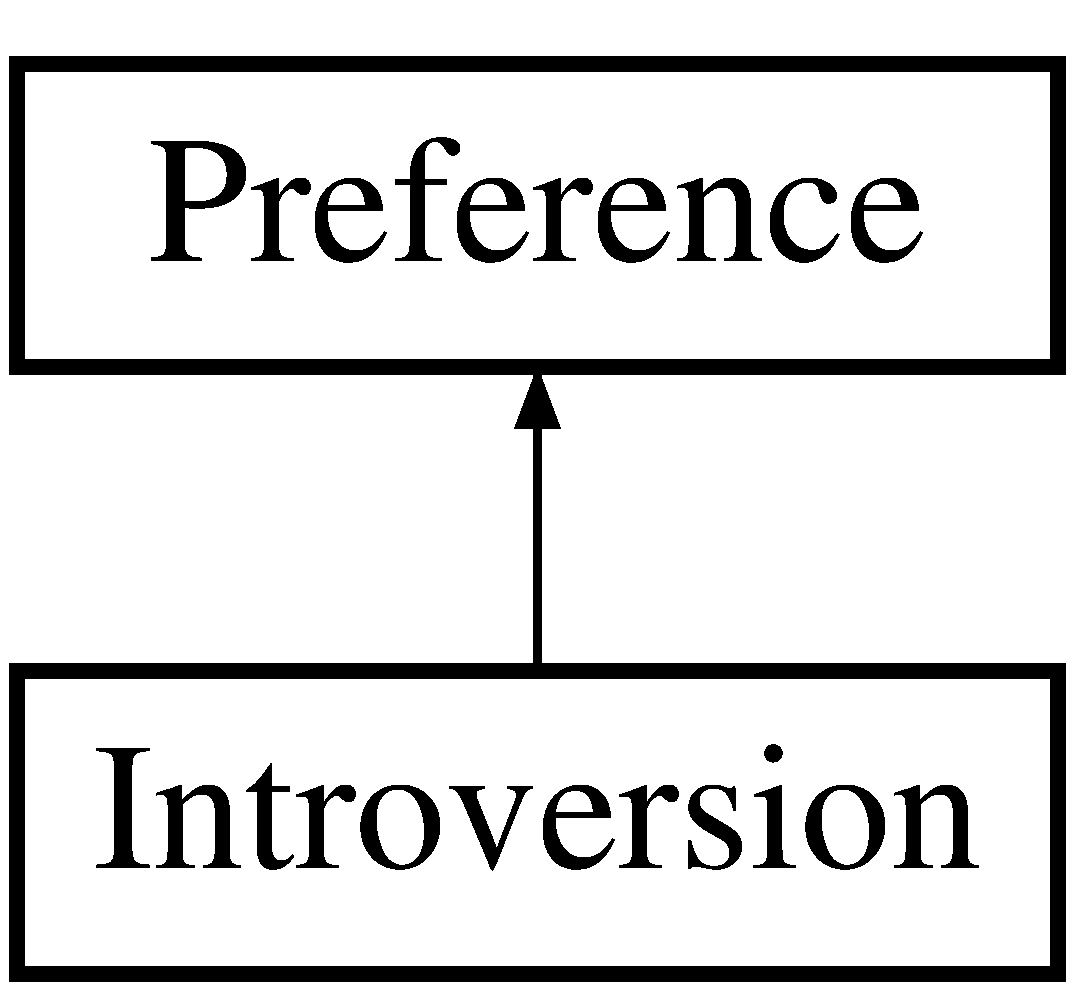
\includegraphics[height=2.000000cm]{class_classes_1_1_preferences_1_1_introversion}
\end{center}
\end{figure}
\subsection*{Data Fields}
\begin{DoxyCompactItemize}
\item 
\hyperlink{class_classes_1_1_preferences_1_1_introversion_aa04ae5f5f106925e87308c0520c0837a}{\$symbol} = \char`\"{}I\char`\"{}
\item 
\hyperlink{class_classes_1_1_preferences_1_1_introversion_ab2fc40d43824ea3e1ce5d86dee0d763b}{\$name} = \char`\"{}Интроверсия\char`\"{}
\item 
\hyperlink{class_classes_1_1_preferences_1_1_introversion_a87b032cba06009e3467abf1c8018d960}{\$description} = \char`\"{}Ориентация сознания внутрь, на субъекта\char`\"{}
\end{DoxyCompactItemize}
\subsection*{Additional Inherited Members}


\subsection{Field Documentation}
\mbox{\Hypertarget{class_classes_1_1_preferences_1_1_introversion_a87b032cba06009e3467abf1c8018d960}\label{class_classes_1_1_preferences_1_1_introversion_a87b032cba06009e3467abf1c8018d960}} 
\index{Classes\+::\+Preferences\+::\+Introversion@{Classes\+::\+Preferences\+::\+Introversion}!\$description@{\$description}}
\index{\$description@{\$description}!Classes\+::\+Preferences\+::\+Introversion@{Classes\+::\+Preferences\+::\+Introversion}}
\subsubsection{\texorpdfstring{\$description}{$description}}
{\footnotesize\ttfamily \$description = \char`\"{}Ориентация сознания внутрь, на субъекта\char`\"{}}

\mbox{\Hypertarget{class_classes_1_1_preferences_1_1_introversion_ab2fc40d43824ea3e1ce5d86dee0d763b}\label{class_classes_1_1_preferences_1_1_introversion_ab2fc40d43824ea3e1ce5d86dee0d763b}} 
\index{Classes\+::\+Preferences\+::\+Introversion@{Classes\+::\+Preferences\+::\+Introversion}!\$name@{\$name}}
\index{\$name@{\$name}!Classes\+::\+Preferences\+::\+Introversion@{Classes\+::\+Preferences\+::\+Introversion}}
\subsubsection{\texorpdfstring{\$name}{$name}}
{\footnotesize\ttfamily \$name = \char`\"{}Интроверсия\char`\"{}}

\mbox{\Hypertarget{class_classes_1_1_preferences_1_1_introversion_aa04ae5f5f106925e87308c0520c0837a}\label{class_classes_1_1_preferences_1_1_introversion_aa04ae5f5f106925e87308c0520c0837a}} 
\index{Classes\+::\+Preferences\+::\+Introversion@{Classes\+::\+Preferences\+::\+Introversion}!\$symbol@{\$symbol}}
\index{\$symbol@{\$symbol}!Classes\+::\+Preferences\+::\+Introversion@{Classes\+::\+Preferences\+::\+Introversion}}
\subsubsection{\texorpdfstring{\$symbol}{$symbol}}
{\footnotesize\ttfamily \$symbol = \char`\"{}I\char`\"{}}



The documentation for this class was generated from the following file\+:\begin{DoxyCompactItemize}
\item 
E\+:/\+Server/\+Open\+Server/domains/localhost/\+M\+B\+T\+I-\/test/\+Classes/\+Preferences/\hyperlink{_introversion_8php}{Introversion.\+php}\end{DoxyCompactItemize}

\hypertarget{class_classes_1_1_preferences_1_1_intuition}{}\section{Intuition Class Reference}
\label{class_classes_1_1_preferences_1_1_intuition}\index{Intuition@{Intuition}}
Inheritance diagram for Intuition\+:\begin{figure}[H]
\begin{center}
\leavevmode
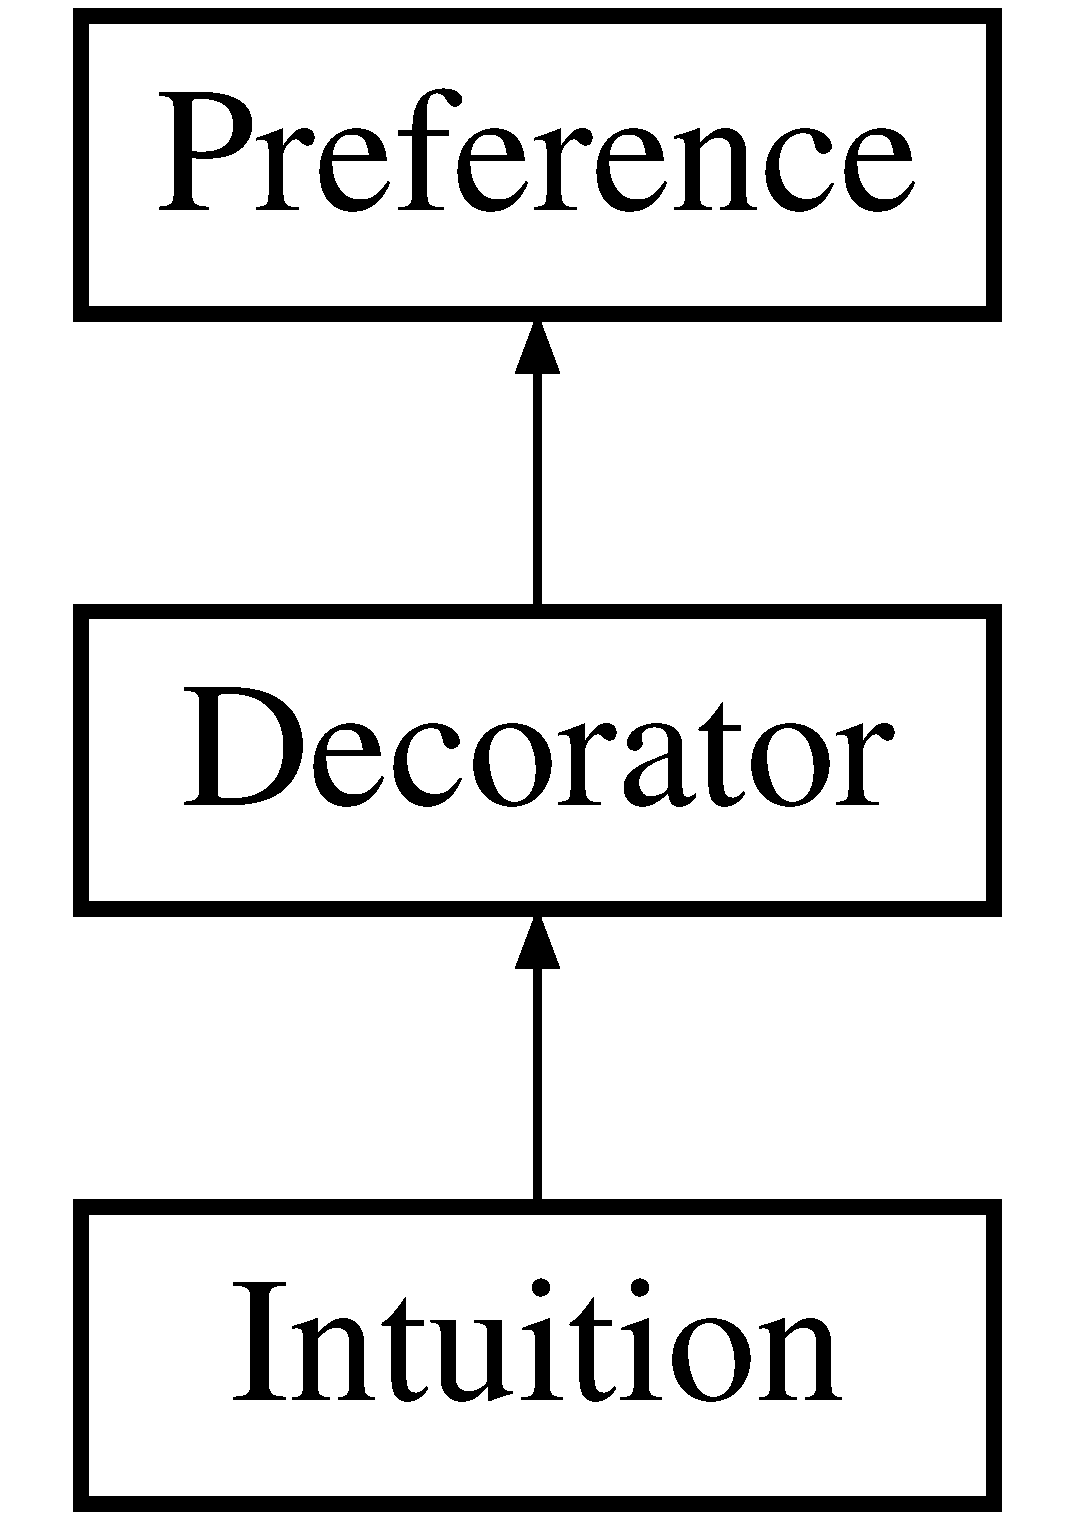
\includegraphics[height=3.000000cm]{class_classes_1_1_preferences_1_1_intuition}
\end{center}
\end{figure}
\subsection*{Data Fields}
\begin{DoxyCompactItemize}
\item 
\hyperlink{class_classes_1_1_preferences_1_1_intuition_aa04ae5f5f106925e87308c0520c0837a}{\$symbol} = \char`\"{}N\char`\"{}
\item 
\hyperlink{class_classes_1_1_preferences_1_1_intuition_ab2fc40d43824ea3e1ce5d86dee0d763b}{\$name} = \char`\"{}Интуиция\char`\"{}
\item 
\hyperlink{class_classes_1_1_preferences_1_1_intuition_a87b032cba06009e3467abf1c8018d960}{\$description} = \char`\"{}Ориентация на оющую, интуитивную информацию\char`\"{}
\end{DoxyCompactItemize}
\subsection*{Additional Inherited Members}


\subsection{Field Documentation}
\mbox{\Hypertarget{class_classes_1_1_preferences_1_1_intuition_a87b032cba06009e3467abf1c8018d960}\label{class_classes_1_1_preferences_1_1_intuition_a87b032cba06009e3467abf1c8018d960}} 
\index{Classes\+::\+Preferences\+::\+Intuition@{Classes\+::\+Preferences\+::\+Intuition}!\$description@{\$description}}
\index{\$description@{\$description}!Classes\+::\+Preferences\+::\+Intuition@{Classes\+::\+Preferences\+::\+Intuition}}
\subsubsection{\texorpdfstring{\$description}{$description}}
{\footnotesize\ttfamily \$description = \char`\"{}Ориентация на оющую, интуитивную информацию\char`\"{}}

\mbox{\Hypertarget{class_classes_1_1_preferences_1_1_intuition_ab2fc40d43824ea3e1ce5d86dee0d763b}\label{class_classes_1_1_preferences_1_1_intuition_ab2fc40d43824ea3e1ce5d86dee0d763b}} 
\index{Classes\+::\+Preferences\+::\+Intuition@{Classes\+::\+Preferences\+::\+Intuition}!\$name@{\$name}}
\index{\$name@{\$name}!Classes\+::\+Preferences\+::\+Intuition@{Classes\+::\+Preferences\+::\+Intuition}}
\subsubsection{\texorpdfstring{\$name}{$name}}
{\footnotesize\ttfamily \$name = \char`\"{}Интуиция\char`\"{}}

\mbox{\Hypertarget{class_classes_1_1_preferences_1_1_intuition_aa04ae5f5f106925e87308c0520c0837a}\label{class_classes_1_1_preferences_1_1_intuition_aa04ae5f5f106925e87308c0520c0837a}} 
\index{Classes\+::\+Preferences\+::\+Intuition@{Classes\+::\+Preferences\+::\+Intuition}!\$symbol@{\$symbol}}
\index{\$symbol@{\$symbol}!Classes\+::\+Preferences\+::\+Intuition@{Classes\+::\+Preferences\+::\+Intuition}}
\subsubsection{\texorpdfstring{\$symbol}{$symbol}}
{\footnotesize\ttfamily \$symbol = \char`\"{}N\char`\"{}}



The documentation for this class was generated from the following file\+:\begin{DoxyCompactItemize}
\item 
E\+:/\+Server/\+Open\+Server/domains/localhost/\+M\+B\+T\+I-\/test/\+Classes/\+Preferences/\hyperlink{_intuition_8php}{Intuition.\+php}\end{DoxyCompactItemize}

\hypertarget{class_classes_1_1_preferences_1_1_judging}{}\section{Judging Class Reference}
\label{class_classes_1_1_preferences_1_1_judging}\index{Judging@{Judging}}
Inheritance diagram for Judging\+:\begin{figure}[H]
\begin{center}
\leavevmode
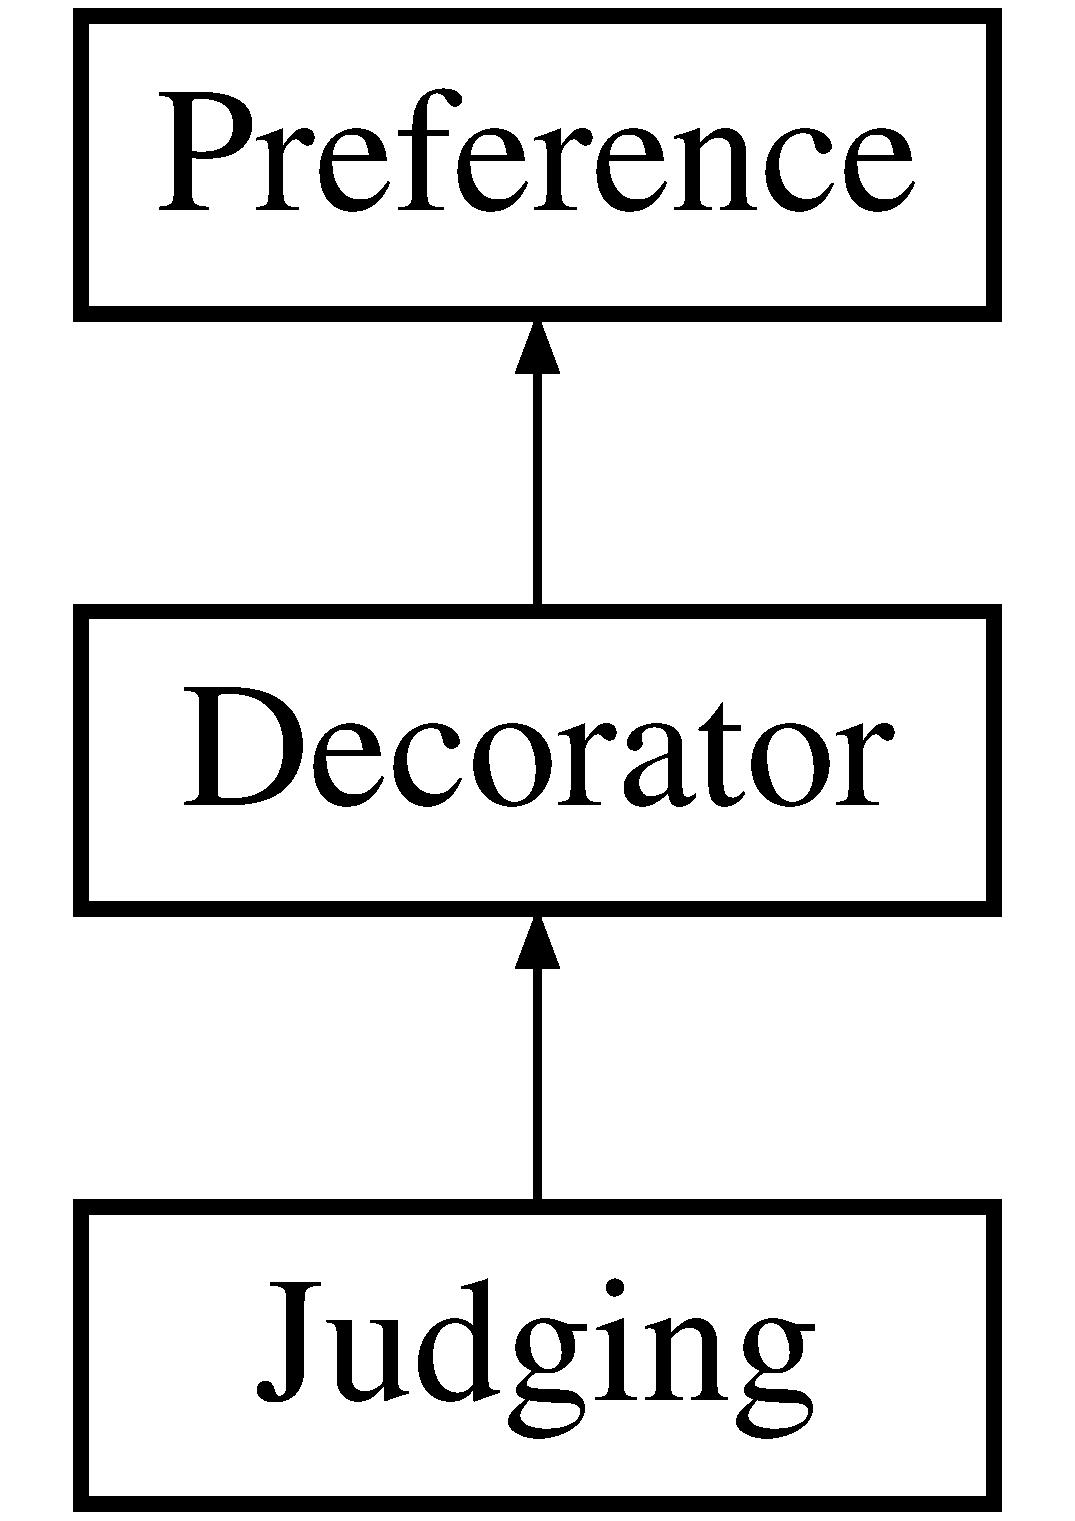
\includegraphics[height=3.000000cm]{class_classes_1_1_preferences_1_1_judging}
\end{center}
\end{figure}
\subsection*{Data Fields}
\begin{DoxyCompactItemize}
\item 
\hyperlink{class_classes_1_1_preferences_1_1_judging_aa04ae5f5f106925e87308c0520c0837a}{\$symbol} = \char`\"{}J\char`\"{}
\item 
\hyperlink{class_classes_1_1_preferences_1_1_judging_ab2fc40d43824ea3e1ce5d86dee0d763b}{\$name} = \char`\"{}Суждение\char`\"{}
\item 
\hyperlink{class_classes_1_1_preferences_1_1_judging_a87b032cba06009e3467abf1c8018d960}{\$description} = \char`\"{}Предпочтение планировать и заранее упорядочивать информацию\char`\"{}
\end{DoxyCompactItemize}
\subsection*{Additional Inherited Members}


\subsection{Field Documentation}
\mbox{\Hypertarget{class_classes_1_1_preferences_1_1_judging_a87b032cba06009e3467abf1c8018d960}\label{class_classes_1_1_preferences_1_1_judging_a87b032cba06009e3467abf1c8018d960}} 
\index{Classes\+::\+Preferences\+::\+Judging@{Classes\+::\+Preferences\+::\+Judging}!\$description@{\$description}}
\index{\$description@{\$description}!Classes\+::\+Preferences\+::\+Judging@{Classes\+::\+Preferences\+::\+Judging}}
\subsubsection{\texorpdfstring{\$description}{$description}}
{\footnotesize\ttfamily \$description = \char`\"{}Предпочтение планировать и заранее упорядочивать информацию\char`\"{}}

\mbox{\Hypertarget{class_classes_1_1_preferences_1_1_judging_ab2fc40d43824ea3e1ce5d86dee0d763b}\label{class_classes_1_1_preferences_1_1_judging_ab2fc40d43824ea3e1ce5d86dee0d763b}} 
\index{Classes\+::\+Preferences\+::\+Judging@{Classes\+::\+Preferences\+::\+Judging}!\$name@{\$name}}
\index{\$name@{\$name}!Classes\+::\+Preferences\+::\+Judging@{Classes\+::\+Preferences\+::\+Judging}}
\subsubsection{\texorpdfstring{\$name}{$name}}
{\footnotesize\ttfamily \$name = \char`\"{}Суждение\char`\"{}}

\mbox{\Hypertarget{class_classes_1_1_preferences_1_1_judging_aa04ae5f5f106925e87308c0520c0837a}\label{class_classes_1_1_preferences_1_1_judging_aa04ae5f5f106925e87308c0520c0837a}} 
\index{Classes\+::\+Preferences\+::\+Judging@{Classes\+::\+Preferences\+::\+Judging}!\$symbol@{\$symbol}}
\index{\$symbol@{\$symbol}!Classes\+::\+Preferences\+::\+Judging@{Classes\+::\+Preferences\+::\+Judging}}
\subsubsection{\texorpdfstring{\$symbol}{$symbol}}
{\footnotesize\ttfamily \$symbol = \char`\"{}J\char`\"{}}



The documentation for this class was generated from the following file\+:\begin{DoxyCompactItemize}
\item 
E\+:/\+Server/\+Open\+Server/domains/localhost/\+M\+B\+T\+I-\/test/\+Classes/\+Preferences/\hyperlink{_judging_8php}{Judging.\+php}\end{DoxyCompactItemize}

\hypertarget{class_classes_1_1_preferences_1_1_perceiving}{}\section{Perceiving Class Reference}
\label{class_classes_1_1_preferences_1_1_perceiving}\index{Perceiving@{Perceiving}}
Inheritance diagram for Perceiving\+:\begin{figure}[H]
\begin{center}
\leavevmode
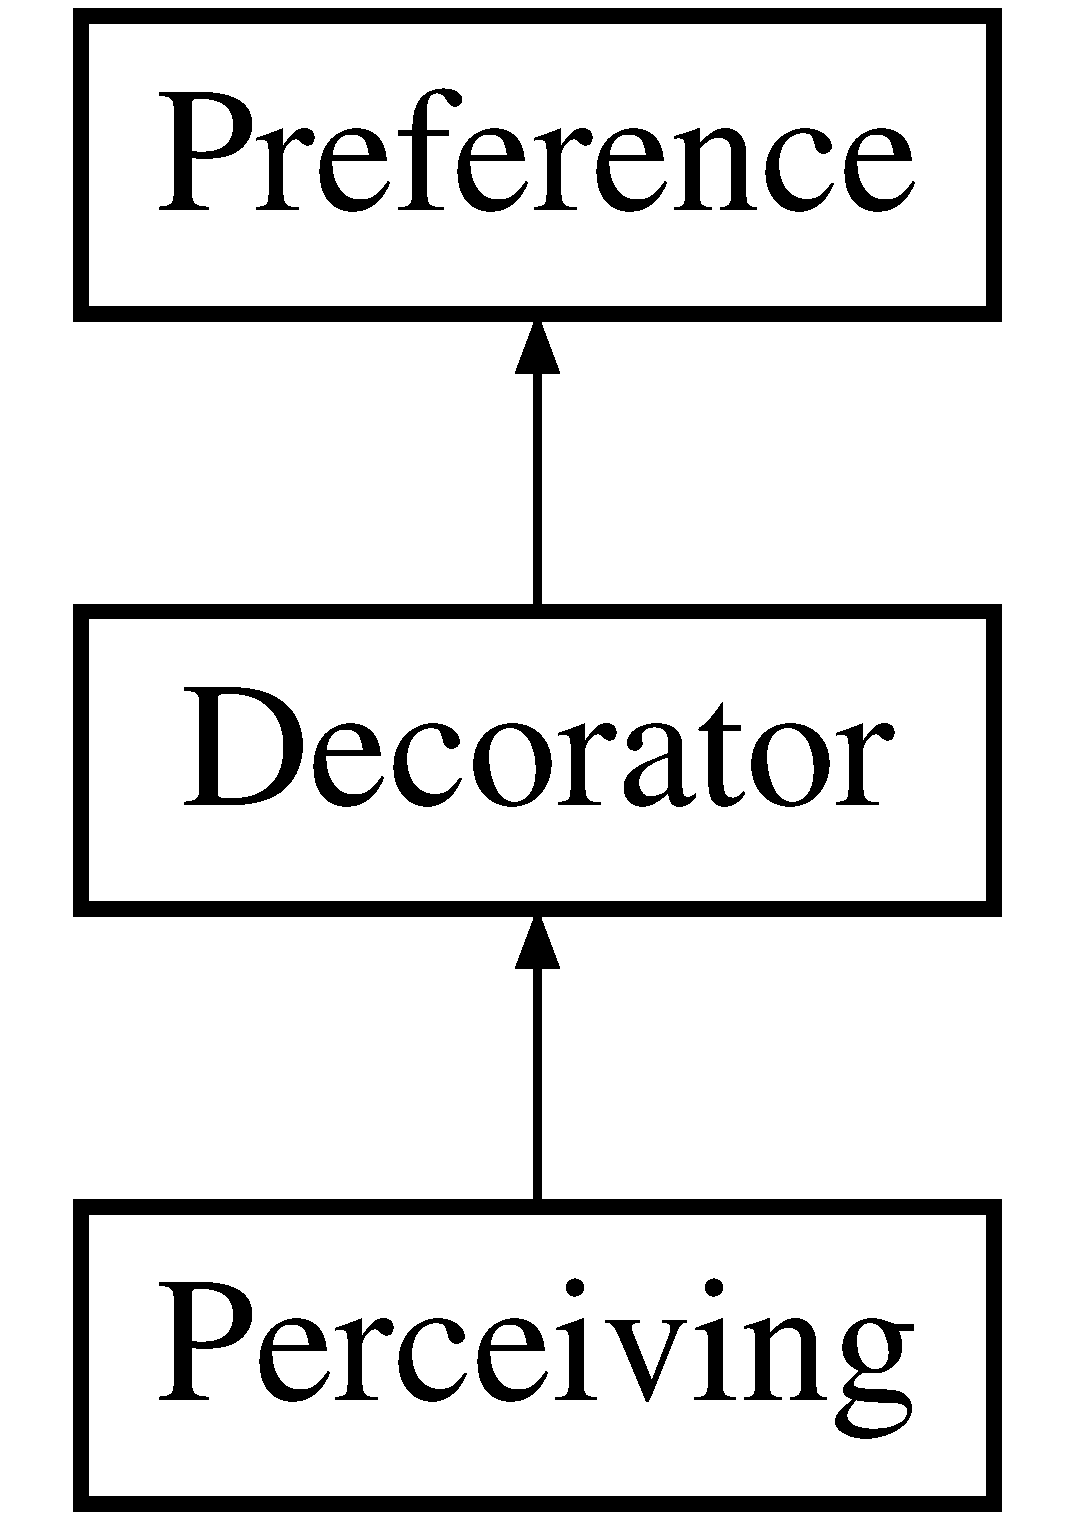
\includegraphics[height=3.000000cm]{class_classes_1_1_preferences_1_1_perceiving}
\end{center}
\end{figure}
\subsection*{Data Fields}
\begin{DoxyCompactItemize}
\item 
\hyperlink{class_classes_1_1_preferences_1_1_perceiving_aa04ae5f5f106925e87308c0520c0837a}{\$symbol} = \char`\"{}P\char`\"{}
\item 
\hyperlink{class_classes_1_1_preferences_1_1_perceiving_ab2fc40d43824ea3e1ce5d86dee0d763b}{\$name} = \char`\"{}Восприятие\char`\"{}
\item 
\hyperlink{class_classes_1_1_preferences_1_1_perceiving_a87b032cba06009e3467abf1c8018d960}{\$description} = \char`\"{}Предпочтение действовать ориентируясь по обстоятельствам\char`\"{}
\end{DoxyCompactItemize}
\subsection*{Additional Inherited Members}


\subsection{Field Documentation}
\mbox{\Hypertarget{class_classes_1_1_preferences_1_1_perceiving_a87b032cba06009e3467abf1c8018d960}\label{class_classes_1_1_preferences_1_1_perceiving_a87b032cba06009e3467abf1c8018d960}} 
\index{Classes\+::\+Preferences\+::\+Perceiving@{Classes\+::\+Preferences\+::\+Perceiving}!\$description@{\$description}}
\index{\$description@{\$description}!Classes\+::\+Preferences\+::\+Perceiving@{Classes\+::\+Preferences\+::\+Perceiving}}
\subsubsection{\texorpdfstring{\$description}{$description}}
{\footnotesize\ttfamily \$description = \char`\"{}Предпочтение действовать ориентируясь по обстоятельствам\char`\"{}}

\mbox{\Hypertarget{class_classes_1_1_preferences_1_1_perceiving_ab2fc40d43824ea3e1ce5d86dee0d763b}\label{class_classes_1_1_preferences_1_1_perceiving_ab2fc40d43824ea3e1ce5d86dee0d763b}} 
\index{Classes\+::\+Preferences\+::\+Perceiving@{Classes\+::\+Preferences\+::\+Perceiving}!\$name@{\$name}}
\index{\$name@{\$name}!Classes\+::\+Preferences\+::\+Perceiving@{Classes\+::\+Preferences\+::\+Perceiving}}
\subsubsection{\texorpdfstring{\$name}{$name}}
{\footnotesize\ttfamily \$name = \char`\"{}Восприятие\char`\"{}}

\mbox{\Hypertarget{class_classes_1_1_preferences_1_1_perceiving_aa04ae5f5f106925e87308c0520c0837a}\label{class_classes_1_1_preferences_1_1_perceiving_aa04ae5f5f106925e87308c0520c0837a}} 
\index{Classes\+::\+Preferences\+::\+Perceiving@{Classes\+::\+Preferences\+::\+Perceiving}!\$symbol@{\$symbol}}
\index{\$symbol@{\$symbol}!Classes\+::\+Preferences\+::\+Perceiving@{Classes\+::\+Preferences\+::\+Perceiving}}
\subsubsection{\texorpdfstring{\$symbol}{$symbol}}
{\footnotesize\ttfamily \$symbol = \char`\"{}P\char`\"{}}



The documentation for this class was generated from the following file\+:\begin{DoxyCompactItemize}
\item 
E\+:/\+Server/\+Open\+Server/domains/localhost/\+M\+B\+T\+I-\/test/\+Classes/\+Preferences/\hyperlink{_perceiving_8php}{Perceiving.\+php}\end{DoxyCompactItemize}

\hypertarget{class_classes_1_1_preferences_1_1_preference}{}\section{Preference Class Reference}
\label{class_classes_1_1_preferences_1_1_preference}\index{Preference@{Preference}}
Inheritance diagram for Preference\+:\begin{figure}[H]
\begin{center}
\leavevmode
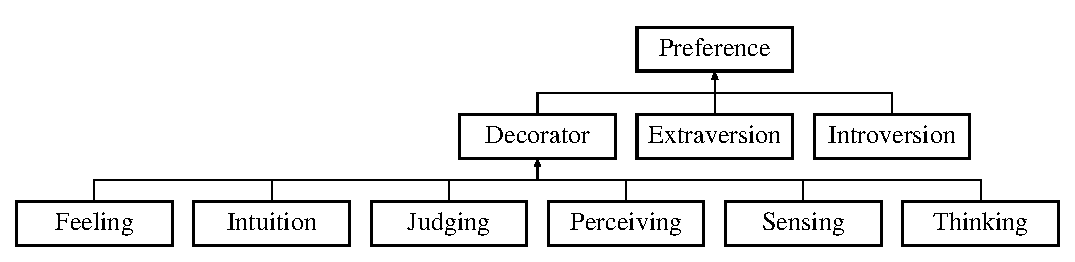
\includegraphics[height=3.000000cm]{class_classes_1_1_preferences_1_1_preference}
\end{center}
\end{figure}
\subsection*{Public Member Functions}
\begin{DoxyCompactItemize}
\item 
\hyperlink{class_classes_1_1_preferences_1_1_preference_a2e7bb35c71bf1824456ceb944cb7a845}{get\+Description} ()
\item 
\hyperlink{class_classes_1_1_preferences_1_1_preference_a830b5c75df72b32396701bc563fbe3c7}{get\+Type} ()
\end{DoxyCompactItemize}
\subsection*{Data Fields}
\begin{DoxyCompactItemize}
\item 
\hyperlink{class_classes_1_1_preferences_1_1_preference_aa04ae5f5f106925e87308c0520c0837a}{\$symbol}
\item 
\hyperlink{class_classes_1_1_preferences_1_1_preference_ab2fc40d43824ea3e1ce5d86dee0d763b}{\$name}
\item 
\hyperlink{class_classes_1_1_preferences_1_1_preference_a87b032cba06009e3467abf1c8018d960}{\$description}
\end{DoxyCompactItemize}


\subsection{Member Function Documentation}
\mbox{\Hypertarget{class_classes_1_1_preferences_1_1_preference_a2e7bb35c71bf1824456ceb944cb7a845}\label{class_classes_1_1_preferences_1_1_preference_a2e7bb35c71bf1824456ceb944cb7a845}} 
\index{Classes\+::\+Preferences\+::\+Preference@{Classes\+::\+Preferences\+::\+Preference}!get\+Description@{get\+Description}}
\index{get\+Description@{get\+Description}!Classes\+::\+Preferences\+::\+Preference@{Classes\+::\+Preferences\+::\+Preference}}
\subsubsection{\texorpdfstring{get\+Description()}{getDescription()}}
{\footnotesize\ttfamily get\+Description (\begin{DoxyParamCaption}{ }\end{DoxyParamCaption})}

\mbox{\Hypertarget{class_classes_1_1_preferences_1_1_preference_a830b5c75df72b32396701bc563fbe3c7}\label{class_classes_1_1_preferences_1_1_preference_a830b5c75df72b32396701bc563fbe3c7}} 
\index{Classes\+::\+Preferences\+::\+Preference@{Classes\+::\+Preferences\+::\+Preference}!get\+Type@{get\+Type}}
\index{get\+Type@{get\+Type}!Classes\+::\+Preferences\+::\+Preference@{Classes\+::\+Preferences\+::\+Preference}}
\subsubsection{\texorpdfstring{get\+Type()}{getType()}}
{\footnotesize\ttfamily get\+Type (\begin{DoxyParamCaption}{ }\end{DoxyParamCaption})}



\subsection{Field Documentation}
\mbox{\Hypertarget{class_classes_1_1_preferences_1_1_preference_a87b032cba06009e3467abf1c8018d960}\label{class_classes_1_1_preferences_1_1_preference_a87b032cba06009e3467abf1c8018d960}} 
\index{Classes\+::\+Preferences\+::\+Preference@{Classes\+::\+Preferences\+::\+Preference}!\$description@{\$description}}
\index{\$description@{\$description}!Classes\+::\+Preferences\+::\+Preference@{Classes\+::\+Preferences\+::\+Preference}}
\subsubsection{\texorpdfstring{\$description}{$description}}
{\footnotesize\ttfamily \$description}

\mbox{\Hypertarget{class_classes_1_1_preferences_1_1_preference_ab2fc40d43824ea3e1ce5d86dee0d763b}\label{class_classes_1_1_preferences_1_1_preference_ab2fc40d43824ea3e1ce5d86dee0d763b}} 
\index{Classes\+::\+Preferences\+::\+Preference@{Classes\+::\+Preferences\+::\+Preference}!\$name@{\$name}}
\index{\$name@{\$name}!Classes\+::\+Preferences\+::\+Preference@{Classes\+::\+Preferences\+::\+Preference}}
\subsubsection{\texorpdfstring{\$name}{$name}}
{\footnotesize\ttfamily \$name}

\mbox{\Hypertarget{class_classes_1_1_preferences_1_1_preference_aa04ae5f5f106925e87308c0520c0837a}\label{class_classes_1_1_preferences_1_1_preference_aa04ae5f5f106925e87308c0520c0837a}} 
\index{Classes\+::\+Preferences\+::\+Preference@{Classes\+::\+Preferences\+::\+Preference}!\$symbol@{\$symbol}}
\index{\$symbol@{\$symbol}!Classes\+::\+Preferences\+::\+Preference@{Classes\+::\+Preferences\+::\+Preference}}
\subsubsection{\texorpdfstring{\$symbol}{$symbol}}
{\footnotesize\ttfamily \$symbol}



The documentation for this class was generated from the following file\+:\begin{DoxyCompactItemize}
\item 
E\+:/\+Server/\+Open\+Server/domains/localhost/\+M\+B\+T\+I-\/test/\+Classes/\+Preferences/\hyperlink{_preference_8php}{Preference.\+php}\end{DoxyCompactItemize}

\hypertarget{class_classes_1_1_test_1_1_question}{}\section{Question Class Reference}
\label{class_classes_1_1_test_1_1_question}\index{Question@{Question}}
\subsection*{Public Member Functions}
\begin{DoxyCompactItemize}
\item 
\hyperlink{class_classes_1_1_test_1_1_question_a26d28169567272deb1df48eff53ed938}{\+\_\+\+\_\+construct} (\$name, \$description, \$reverse=false)
\item 
\hyperlink{class_classes_1_1_test_1_1_question_a2e7bb35c71bf1824456ceb944cb7a845}{get\+Description} ()
\item 
\hyperlink{class_classes_1_1_test_1_1_question_a3d0963e68bb313b163a73f2803c64600}{get\+Name} ()
\item 
\hyperlink{class_classes_1_1_test_1_1_question_a5a580ca3aa63e02e3f7907ac10c2f5d6}{get\+Reverse} ()
\end{DoxyCompactItemize}


\subsection{Constructor \& Destructor Documentation}
\mbox{\Hypertarget{class_classes_1_1_test_1_1_question_a26d28169567272deb1df48eff53ed938}\label{class_classes_1_1_test_1_1_question_a26d28169567272deb1df48eff53ed938}} 
\index{Classes\+::\+Test\+::\+Question@{Classes\+::\+Test\+::\+Question}!\+\_\+\+\_\+construct@{\+\_\+\+\_\+construct}}
\index{\+\_\+\+\_\+construct@{\+\_\+\+\_\+construct}!Classes\+::\+Test\+::\+Question@{Classes\+::\+Test\+::\+Question}}
\subsubsection{\texorpdfstring{\+\_\+\+\_\+construct()}{\_\_construct()}}
{\footnotesize\ttfamily \+\_\+\+\_\+construct (\begin{DoxyParamCaption}\item[{}]{\$name,  }\item[{}]{\$description,  }\item[{}]{\$reverse = {\ttfamily false} }\end{DoxyParamCaption})}



\subsection{Member Function Documentation}
\mbox{\Hypertarget{class_classes_1_1_test_1_1_question_a2e7bb35c71bf1824456ceb944cb7a845}\label{class_classes_1_1_test_1_1_question_a2e7bb35c71bf1824456ceb944cb7a845}} 
\index{Classes\+::\+Test\+::\+Question@{Classes\+::\+Test\+::\+Question}!get\+Description@{get\+Description}}
\index{get\+Description@{get\+Description}!Classes\+::\+Test\+::\+Question@{Classes\+::\+Test\+::\+Question}}
\subsubsection{\texorpdfstring{get\+Description()}{getDescription()}}
{\footnotesize\ttfamily get\+Description (\begin{DoxyParamCaption}{ }\end{DoxyParamCaption})}

\mbox{\Hypertarget{class_classes_1_1_test_1_1_question_a3d0963e68bb313b163a73f2803c64600}\label{class_classes_1_1_test_1_1_question_a3d0963e68bb313b163a73f2803c64600}} 
\index{Classes\+::\+Test\+::\+Question@{Classes\+::\+Test\+::\+Question}!get\+Name@{get\+Name}}
\index{get\+Name@{get\+Name}!Classes\+::\+Test\+::\+Question@{Classes\+::\+Test\+::\+Question}}
\subsubsection{\texorpdfstring{get\+Name()}{getName()}}
{\footnotesize\ttfamily get\+Name (\begin{DoxyParamCaption}{ }\end{DoxyParamCaption})}

\mbox{\Hypertarget{class_classes_1_1_test_1_1_question_a5a580ca3aa63e02e3f7907ac10c2f5d6}\label{class_classes_1_1_test_1_1_question_a5a580ca3aa63e02e3f7907ac10c2f5d6}} 
\index{Classes\+::\+Test\+::\+Question@{Classes\+::\+Test\+::\+Question}!get\+Reverse@{get\+Reverse}}
\index{get\+Reverse@{get\+Reverse}!Classes\+::\+Test\+::\+Question@{Classes\+::\+Test\+::\+Question}}
\subsubsection{\texorpdfstring{get\+Reverse()}{getReverse()}}
{\footnotesize\ttfamily get\+Reverse (\begin{DoxyParamCaption}{ }\end{DoxyParamCaption})}



The documentation for this class was generated from the following file\+:\begin{DoxyCompactItemize}
\item 
E\+:/\+Server/\+Open\+Server/domains/localhost/\+M\+B\+T\+I-\/test/\+Classes/\+Test/\hyperlink{_question_8php}{Question.\+php}\end{DoxyCompactItemize}

\hypertarget{class_classes_1_1_preferences_1_1_sensing}{}\section{Sensing Class Reference}
\label{class_classes_1_1_preferences_1_1_sensing}\index{Sensing@{Sensing}}
Inheritance diagram for Sensing\+:\begin{figure}[H]
\begin{center}
\leavevmode
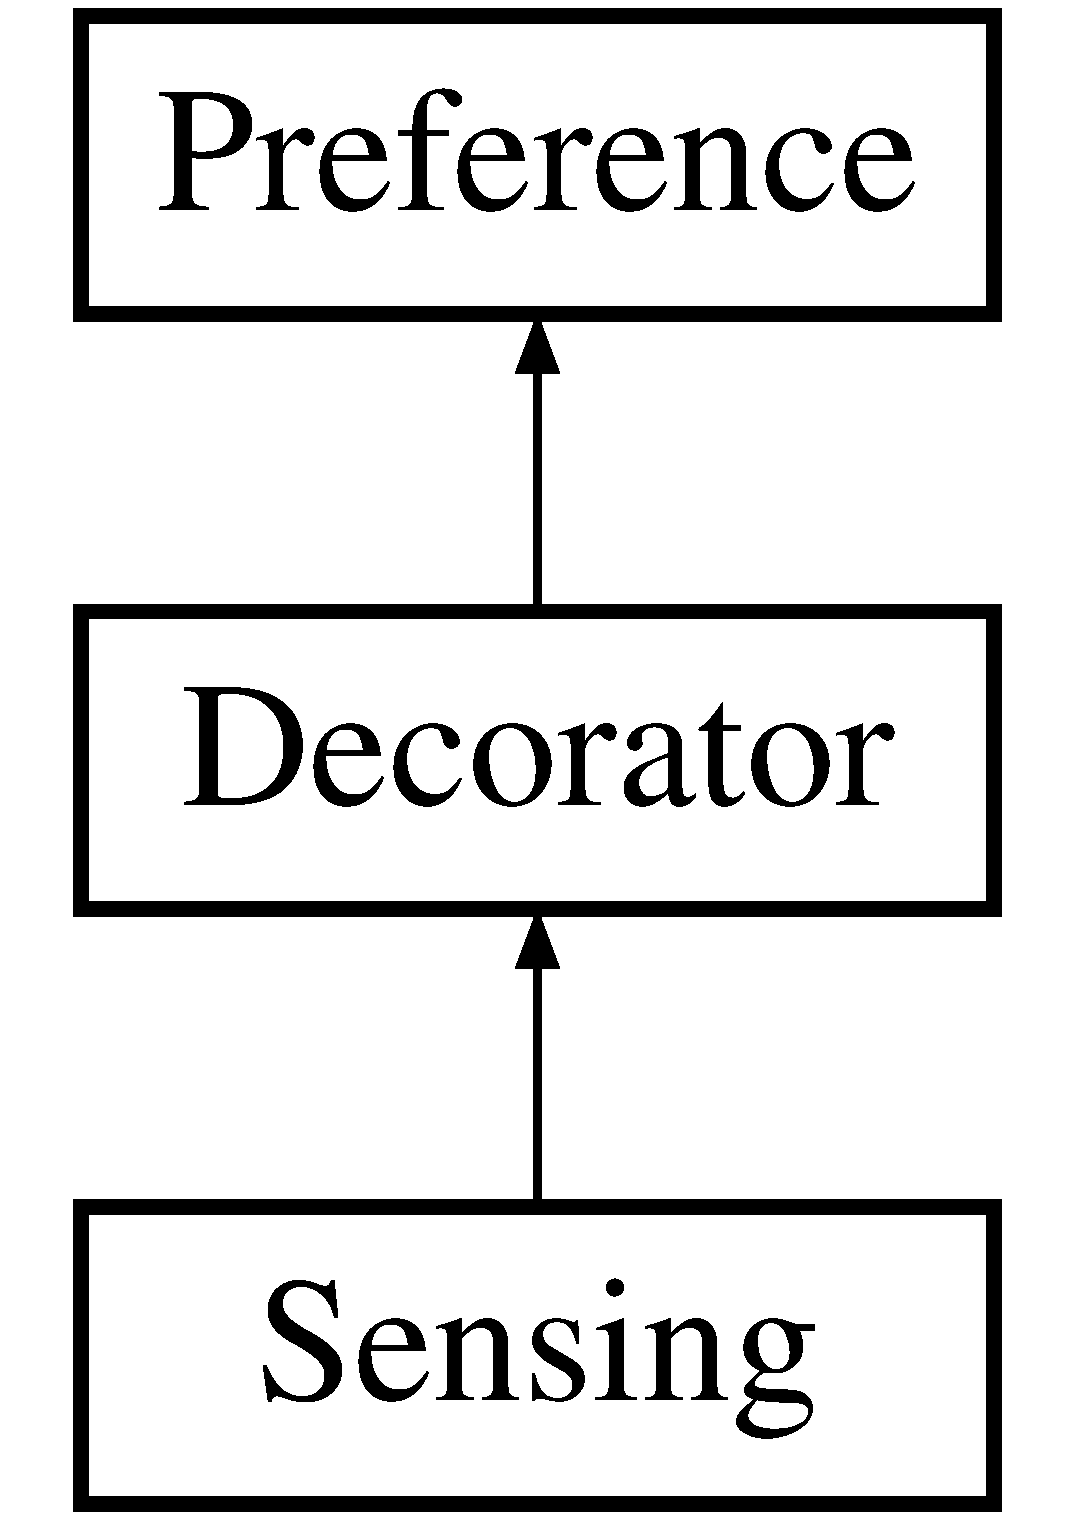
\includegraphics[height=3.000000cm]{class_classes_1_1_preferences_1_1_sensing}
\end{center}
\end{figure}
\subsection*{Data Fields}
\begin{DoxyCompactItemize}
\item 
\hyperlink{class_classes_1_1_preferences_1_1_sensing_aa04ae5f5f106925e87308c0520c0837a}{\$symbol} = \char`\"{}S\char`\"{}
\item 
\hyperlink{class_classes_1_1_preferences_1_1_sensing_ab2fc40d43824ea3e1ce5d86dee0d763b}{\$name} = \char`\"{}Ощущение\char`\"{}
\item 
\hyperlink{class_classes_1_1_preferences_1_1_sensing_a87b032cba06009e3467abf1c8018d960}{\$description} = \char`\"{}Ориентировка на материальную информацию\char`\"{}
\end{DoxyCompactItemize}
\subsection*{Additional Inherited Members}


\subsection{Field Documentation}
\mbox{\Hypertarget{class_classes_1_1_preferences_1_1_sensing_a87b032cba06009e3467abf1c8018d960}\label{class_classes_1_1_preferences_1_1_sensing_a87b032cba06009e3467abf1c8018d960}} 
\index{Classes\+::\+Preferences\+::\+Sensing@{Classes\+::\+Preferences\+::\+Sensing}!\$description@{\$description}}
\index{\$description@{\$description}!Classes\+::\+Preferences\+::\+Sensing@{Classes\+::\+Preferences\+::\+Sensing}}
\subsubsection{\texorpdfstring{\$description}{$description}}
{\footnotesize\ttfamily \$description = \char`\"{}Ориентировка на материальную информацию\char`\"{}}

\mbox{\Hypertarget{class_classes_1_1_preferences_1_1_sensing_ab2fc40d43824ea3e1ce5d86dee0d763b}\label{class_classes_1_1_preferences_1_1_sensing_ab2fc40d43824ea3e1ce5d86dee0d763b}} 
\index{Classes\+::\+Preferences\+::\+Sensing@{Classes\+::\+Preferences\+::\+Sensing}!\$name@{\$name}}
\index{\$name@{\$name}!Classes\+::\+Preferences\+::\+Sensing@{Classes\+::\+Preferences\+::\+Sensing}}
\subsubsection{\texorpdfstring{\$name}{$name}}
{\footnotesize\ttfamily \$name = \char`\"{}Ощущение\char`\"{}}

\mbox{\Hypertarget{class_classes_1_1_preferences_1_1_sensing_aa04ae5f5f106925e87308c0520c0837a}\label{class_classes_1_1_preferences_1_1_sensing_aa04ae5f5f106925e87308c0520c0837a}} 
\index{Classes\+::\+Preferences\+::\+Sensing@{Classes\+::\+Preferences\+::\+Sensing}!\$symbol@{\$symbol}}
\index{\$symbol@{\$symbol}!Classes\+::\+Preferences\+::\+Sensing@{Classes\+::\+Preferences\+::\+Sensing}}
\subsubsection{\texorpdfstring{\$symbol}{$symbol}}
{\footnotesize\ttfamily \$symbol = \char`\"{}S\char`\"{}}



The documentation for this class was generated from the following file\+:\begin{DoxyCompactItemize}
\item 
E\+:/\+Server/\+Open\+Server/domains/localhost/\+M\+B\+T\+I-\/test/\+Classes/\+Preferences/\hyperlink{_sensing_8php}{Sensing.\+php}\end{DoxyCompactItemize}

\hypertarget{class_classes_1_1_test_1_1_set}{}\section{Set Class Reference}
\label{class_classes_1_1_test_1_1_set}\index{Set@{Set}}
\subsection*{Public Member Functions}
\begin{DoxyCompactItemize}
\item 
\hyperlink{class_classes_1_1_test_1_1_set_a095c5d389db211932136b53f25f39685}{\+\_\+\+\_\+construct} ()
\item 
\hyperlink{class_classes_1_1_test_1_1_set_aa27ea8191c7601c3811568b55f9e4c14}{add\+Question} (\hyperlink{class_classes_1_1_test_1_1_question}{Question} \$question)
\item 
\hyperlink{class_classes_1_1_test_1_1_set_aa5473162875f6946182770047be563d7}{get\+Questions} ()
\end{DoxyCompactItemize}


\subsection{Constructor \& Destructor Documentation}
\mbox{\Hypertarget{class_classes_1_1_test_1_1_set_a095c5d389db211932136b53f25f39685}\label{class_classes_1_1_test_1_1_set_a095c5d389db211932136b53f25f39685}} 
\index{Classes\+::\+Test\+::\+Set@{Classes\+::\+Test\+::\+Set}!\+\_\+\+\_\+construct@{\+\_\+\+\_\+construct}}
\index{\+\_\+\+\_\+construct@{\+\_\+\+\_\+construct}!Classes\+::\+Test\+::\+Set@{Classes\+::\+Test\+::\+Set}}
\subsubsection{\texorpdfstring{\+\_\+\+\_\+construct()}{\_\_construct()}}
{\footnotesize\ttfamily \+\_\+\+\_\+construct (\begin{DoxyParamCaption}{ }\end{DoxyParamCaption})}



\subsection{Member Function Documentation}
\mbox{\Hypertarget{class_classes_1_1_test_1_1_set_aa27ea8191c7601c3811568b55f9e4c14}\label{class_classes_1_1_test_1_1_set_aa27ea8191c7601c3811568b55f9e4c14}} 
\index{Classes\+::\+Test\+::\+Set@{Classes\+::\+Test\+::\+Set}!add\+Question@{add\+Question}}
\index{add\+Question@{add\+Question}!Classes\+::\+Test\+::\+Set@{Classes\+::\+Test\+::\+Set}}
\subsubsection{\texorpdfstring{add\+Question()}{addQuestion()}}
{\footnotesize\ttfamily add\+Question (\begin{DoxyParamCaption}\item[{\hyperlink{class_classes_1_1_test_1_1_question}{Question}}]{\$question }\end{DoxyParamCaption})}

\mbox{\Hypertarget{class_classes_1_1_test_1_1_set_aa5473162875f6946182770047be563d7}\label{class_classes_1_1_test_1_1_set_aa5473162875f6946182770047be563d7}} 
\index{Classes\+::\+Test\+::\+Set@{Classes\+::\+Test\+::\+Set}!get\+Questions@{get\+Questions}}
\index{get\+Questions@{get\+Questions}!Classes\+::\+Test\+::\+Set@{Classes\+::\+Test\+::\+Set}}
\subsubsection{\texorpdfstring{get\+Questions()}{getQuestions()}}
{\footnotesize\ttfamily get\+Questions (\begin{DoxyParamCaption}{ }\end{DoxyParamCaption})}



The documentation for this class was generated from the following file\+:\begin{DoxyCompactItemize}
\item 
E\+:/\+Server/\+Open\+Server/domains/localhost/\+M\+B\+T\+I-\/test/\+Classes/\+Test/\hyperlink{_set_8php}{Set.\+php}\end{DoxyCompactItemize}

\hypertarget{class_classes_1_1_test_1_1_test}{}\section{Test Class Reference}
\label{class_classes_1_1_test_1_1_test}\index{Test@{Test}}
\subsection*{Public Member Functions}
\begin{DoxyCompactItemize}
\item 
\hyperlink{class_classes_1_1_test_1_1_test_ae6708de96ea5a340ae2bb47f73c1b990}{add\+Set} (\hyperlink{class_classes_1_1_test_1_1_set}{Set} \$set)
\item 
\hyperlink{class_classes_1_1_test_1_1_test_ae077eb8a032a325ceb939bfabfa5f472}{get\+Result} ()
\item 
\hyperlink{class_classes_1_1_test_1_1_test_a9af17f39a73d4e6194209ba95f557e0a}{get\+Test} ()
\end{DoxyCompactItemize}


\subsection{Member Function Documentation}
\mbox{\Hypertarget{class_classes_1_1_test_1_1_test_ae6708de96ea5a340ae2bb47f73c1b990}\label{class_classes_1_1_test_1_1_test_ae6708de96ea5a340ae2bb47f73c1b990}} 
\index{Classes\+::\+Test\+::\+Test@{Classes\+::\+Test\+::\+Test}!add\+Set@{add\+Set}}
\index{add\+Set@{add\+Set}!Classes\+::\+Test\+::\+Test@{Classes\+::\+Test\+::\+Test}}
\subsubsection{\texorpdfstring{add\+Set()}{addSet()}}
{\footnotesize\ttfamily add\+Set (\begin{DoxyParamCaption}\item[{\hyperlink{class_classes_1_1_test_1_1_set}{Set}}]{\$set }\end{DoxyParamCaption})}

\mbox{\Hypertarget{class_classes_1_1_test_1_1_test_ae077eb8a032a325ceb939bfabfa5f472}\label{class_classes_1_1_test_1_1_test_ae077eb8a032a325ceb939bfabfa5f472}} 
\index{Classes\+::\+Test\+::\+Test@{Classes\+::\+Test\+::\+Test}!get\+Result@{get\+Result}}
\index{get\+Result@{get\+Result}!Classes\+::\+Test\+::\+Test@{Classes\+::\+Test\+::\+Test}}
\subsubsection{\texorpdfstring{get\+Result()}{getResult()}}
{\footnotesize\ttfamily get\+Result (\begin{DoxyParamCaption}{ }\end{DoxyParamCaption})}

\mbox{\Hypertarget{class_classes_1_1_test_1_1_test_a9af17f39a73d4e6194209ba95f557e0a}\label{class_classes_1_1_test_1_1_test_a9af17f39a73d4e6194209ba95f557e0a}} 
\index{Classes\+::\+Test\+::\+Test@{Classes\+::\+Test\+::\+Test}!get\+Test@{get\+Test}}
\index{get\+Test@{get\+Test}!Classes\+::\+Test\+::\+Test@{Classes\+::\+Test\+::\+Test}}
\subsubsection{\texorpdfstring{get\+Test()}{getTest()}}
{\footnotesize\ttfamily get\+Test (\begin{DoxyParamCaption}{ }\end{DoxyParamCaption})}



The documentation for this class was generated from the following file\+:\begin{DoxyCompactItemize}
\item 
E\+:/\+Server/\+Open\+Server/domains/localhost/\+M\+B\+T\+I-\/test/\+Classes/\+Test/\hyperlink{_classes_2_test_2_test_8php}{Test.\+php}\end{DoxyCompactItemize}

\hypertarget{class_classes_1_1_preferences_1_1_thinking}{}\section{Thinking Class Reference}
\label{class_classes_1_1_preferences_1_1_thinking}\index{Thinking@{Thinking}}
Inheritance diagram for Thinking\+:\begin{figure}[H]
\begin{center}
\leavevmode
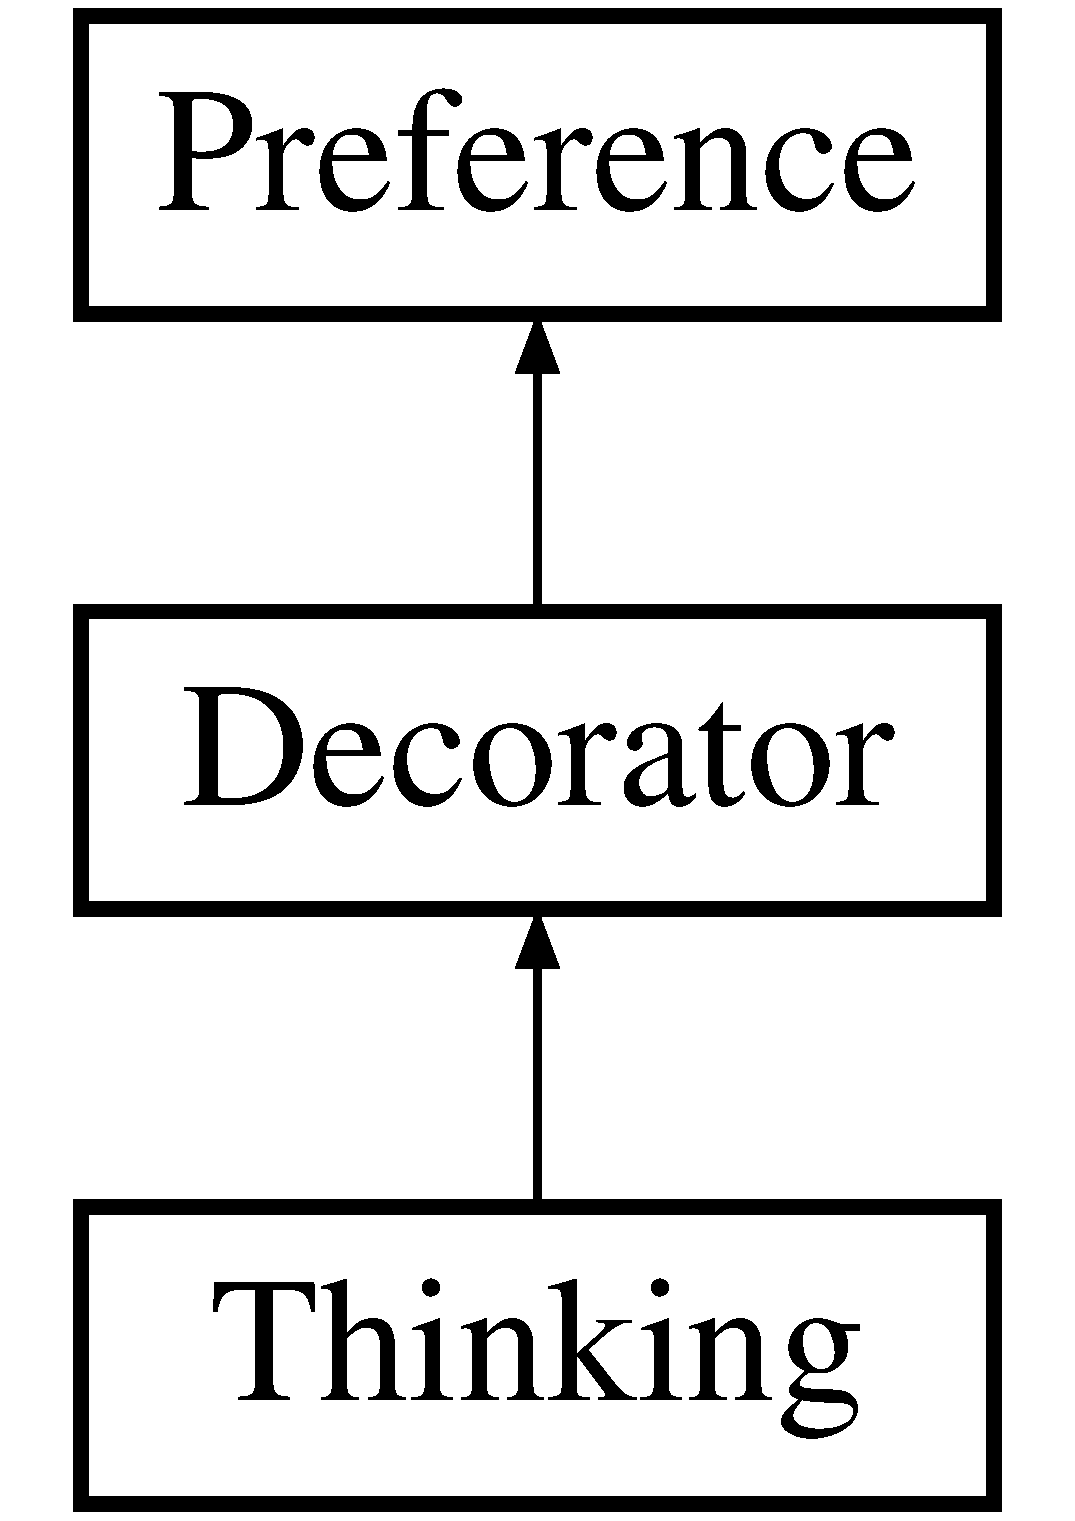
\includegraphics[height=3.000000cm]{class_classes_1_1_preferences_1_1_thinking}
\end{center}
\end{figure}
\subsection*{Data Fields}
\begin{DoxyCompactItemize}
\item 
\hyperlink{class_classes_1_1_preferences_1_1_thinking_aa04ae5f5f106925e87308c0520c0837a}{\$symbol} = \char`\"{}T\char`\"{}
\item 
\hyperlink{class_classes_1_1_preferences_1_1_thinking_ab2fc40d43824ea3e1ce5d86dee0d763b}{\$name} = \char`\"{}Мышление\char`\"{}
\item 
\hyperlink{class_classes_1_1_preferences_1_1_thinking_a87b032cba06009e3467abf1c8018d960}{\$description} = \char`\"{}Рациональное взвешивание альтернатив\char`\"{}
\end{DoxyCompactItemize}
\subsection*{Additional Inherited Members}


\subsection{Field Documentation}
\mbox{\Hypertarget{class_classes_1_1_preferences_1_1_thinking_a87b032cba06009e3467abf1c8018d960}\label{class_classes_1_1_preferences_1_1_thinking_a87b032cba06009e3467abf1c8018d960}} 
\index{Classes\+::\+Preferences\+::\+Thinking@{Classes\+::\+Preferences\+::\+Thinking}!\$description@{\$description}}
\index{\$description@{\$description}!Classes\+::\+Preferences\+::\+Thinking@{Classes\+::\+Preferences\+::\+Thinking}}
\subsubsection{\texorpdfstring{\$description}{$description}}
{\footnotesize\ttfamily \$description = \char`\"{}Рациональное взвешивание альтернатив\char`\"{}}

\mbox{\Hypertarget{class_classes_1_1_preferences_1_1_thinking_ab2fc40d43824ea3e1ce5d86dee0d763b}\label{class_classes_1_1_preferences_1_1_thinking_ab2fc40d43824ea3e1ce5d86dee0d763b}} 
\index{Classes\+::\+Preferences\+::\+Thinking@{Classes\+::\+Preferences\+::\+Thinking}!\$name@{\$name}}
\index{\$name@{\$name}!Classes\+::\+Preferences\+::\+Thinking@{Classes\+::\+Preferences\+::\+Thinking}}
\subsubsection{\texorpdfstring{\$name}{$name}}
{\footnotesize\ttfamily \$name = \char`\"{}Мышление\char`\"{}}

\mbox{\Hypertarget{class_classes_1_1_preferences_1_1_thinking_aa04ae5f5f106925e87308c0520c0837a}\label{class_classes_1_1_preferences_1_1_thinking_aa04ae5f5f106925e87308c0520c0837a}} 
\index{Classes\+::\+Preferences\+::\+Thinking@{Classes\+::\+Preferences\+::\+Thinking}!\$symbol@{\$symbol}}
\index{\$symbol@{\$symbol}!Classes\+::\+Preferences\+::\+Thinking@{Classes\+::\+Preferences\+::\+Thinking}}
\subsubsection{\texorpdfstring{\$symbol}{$symbol}}
{\footnotesize\ttfamily \$symbol = \char`\"{}T\char`\"{}}



The documentation for this class was generated from the following file\+:\begin{DoxyCompactItemize}
\item 
E\+:/\+Server/\+Open\+Server/domains/localhost/\+M\+B\+T\+I-\/test/\+Classes/\+Preferences/\hyperlink{_thinking_8php}{Thinking.\+php}\end{DoxyCompactItemize}

\hypertarget{class_classes_1_1_types_1_1_type}{}\section{Type Class Reference}
\label{class_classes_1_1_types_1_1_type}\index{Type@{Type}}
\subsection*{Public Member Functions}
\begin{DoxyCompactItemize}
\item 
\hyperlink{class_classes_1_1_types_1_1_type_a486200d625fce8d389146cafb948bb11}{\+\_\+\+\_\+construct} (\$arr)
\item 
\hyperlink{class_classes_1_1_types_1_1_type_a71d04ef07804d67e24e87339e00d8446}{set\+Functions} (\hyperlink{class_classes_1_1_preferences_1_1_preference}{Preference} \$functions)
\item 
\hyperlink{class_classes_1_1_types_1_1_type_a2e7bb35c71bf1824456ceb944cb7a845}{get\+Description} ()
\end{DoxyCompactItemize}


\subsection{Constructor \& Destructor Documentation}
\mbox{\Hypertarget{class_classes_1_1_types_1_1_type_a486200d625fce8d389146cafb948bb11}\label{class_classes_1_1_types_1_1_type_a486200d625fce8d389146cafb948bb11}} 
\index{Classes\+::\+Types\+::\+Type@{Classes\+::\+Types\+::\+Type}!\+\_\+\+\_\+construct@{\+\_\+\+\_\+construct}}
\index{\+\_\+\+\_\+construct@{\+\_\+\+\_\+construct}!Classes\+::\+Types\+::\+Type@{Classes\+::\+Types\+::\+Type}}
\subsubsection{\texorpdfstring{\+\_\+\+\_\+construct()}{\_\_construct()}}
{\footnotesize\ttfamily \+\_\+\+\_\+construct (\begin{DoxyParamCaption}\item[{}]{\$arr }\end{DoxyParamCaption})}



\subsection{Member Function Documentation}
\mbox{\Hypertarget{class_classes_1_1_types_1_1_type_a2e7bb35c71bf1824456ceb944cb7a845}\label{class_classes_1_1_types_1_1_type_a2e7bb35c71bf1824456ceb944cb7a845}} 
\index{Classes\+::\+Types\+::\+Type@{Classes\+::\+Types\+::\+Type}!get\+Description@{get\+Description}}
\index{get\+Description@{get\+Description}!Classes\+::\+Types\+::\+Type@{Classes\+::\+Types\+::\+Type}}
\subsubsection{\texorpdfstring{get\+Description()}{getDescription()}}
{\footnotesize\ttfamily get\+Description (\begin{DoxyParamCaption}{ }\end{DoxyParamCaption})}

\mbox{\Hypertarget{class_classes_1_1_types_1_1_type_a71d04ef07804d67e24e87339e00d8446}\label{class_classes_1_1_types_1_1_type_a71d04ef07804d67e24e87339e00d8446}} 
\index{Classes\+::\+Types\+::\+Type@{Classes\+::\+Types\+::\+Type}!set\+Functions@{set\+Functions}}
\index{set\+Functions@{set\+Functions}!Classes\+::\+Types\+::\+Type@{Classes\+::\+Types\+::\+Type}}
\subsubsection{\texorpdfstring{set\+Functions()}{setFunctions()}}
{\footnotesize\ttfamily set\+Functions (\begin{DoxyParamCaption}\item[{\hyperlink{class_classes_1_1_preferences_1_1_preference}{Preference}}]{\$functions }\end{DoxyParamCaption})}



The documentation for this class was generated from the following file\+:\begin{DoxyCompactItemize}
\item 
E\+:/\+Server/\+Open\+Server/domains/localhost/\+M\+B\+T\+I-\/test/\+Classes/\+Types/\hyperlink{_type_8php}{Type.\+php}\end{DoxyCompactItemize}

\chapter{File Documentation}
\hypertarget{_decorator_8php}{}\section{E\+:/\+Server/\+Open\+Server/domains/localhost/\+M\+B\+T\+I-\/test/\+Classes/\+Preferences/\+Decorator.php File Reference}
\label{_decorator_8php}\index{E\+:/\+Server/\+Open\+Server/domains/localhost/\+M\+B\+T\+I-\/test/\+Classes/\+Preferences/\+Decorator.\+php@{E\+:/\+Server/\+Open\+Server/domains/localhost/\+M\+B\+T\+I-\/test/\+Classes/\+Preferences/\+Decorator.\+php}}
\subsection*{Data Structures}
\begin{DoxyCompactItemize}
\item 
class \hyperlink{class_classes_1_1_preferences_1_1_decorator}{Decorator}
\end{DoxyCompactItemize}
\subsection*{Namespaces}
\begin{DoxyCompactItemize}
\item 
 \hyperlink{namespace_classes_1_1_preferences}{Classes\textbackslash{}\+Preferences}
\end{DoxyCompactItemize}

\hypertarget{_extraversion_8php}{}\section{E\+:/\+Server/\+Open\+Server/domains/localhost/\+M\+B\+T\+I-\/test/\+Classes/\+Preferences/\+Extraversion.php File Reference}
\label{_extraversion_8php}\index{E\+:/\+Server/\+Open\+Server/domains/localhost/\+M\+B\+T\+I-\/test/\+Classes/\+Preferences/\+Extraversion.\+php@{E\+:/\+Server/\+Open\+Server/domains/localhost/\+M\+B\+T\+I-\/test/\+Classes/\+Preferences/\+Extraversion.\+php}}
\subsection*{Data Structures}
\begin{DoxyCompactItemize}
\item 
class \hyperlink{class_classes_1_1_preferences_1_1_extraversion}{Extraversion}
\end{DoxyCompactItemize}
\subsection*{Namespaces}
\begin{DoxyCompactItemize}
\item 
 \hyperlink{namespace_classes_1_1_preferences}{Classes\textbackslash{}\+Preferences}
\end{DoxyCompactItemize}

\hypertarget{_feeling_8php}{}\section{E\+:/\+Server/\+Open\+Server/domains/localhost/\+M\+B\+T\+I-\/test/\+Classes/\+Preferences/\+Feeling.php File Reference}
\label{_feeling_8php}\index{E\+:/\+Server/\+Open\+Server/domains/localhost/\+M\+B\+T\+I-\/test/\+Classes/\+Preferences/\+Feeling.\+php@{E\+:/\+Server/\+Open\+Server/domains/localhost/\+M\+B\+T\+I-\/test/\+Classes/\+Preferences/\+Feeling.\+php}}
\subsection*{Data Structures}
\begin{DoxyCompactItemize}
\item 
class \hyperlink{class_classes_1_1_preferences_1_1_feeling}{Feeling}
\end{DoxyCompactItemize}
\subsection*{Namespaces}
\begin{DoxyCompactItemize}
\item 
 \hyperlink{namespace_classes_1_1_preferences}{Classes\textbackslash{}\+Preferences}
\end{DoxyCompactItemize}

\hypertarget{_introversion_8php}{}\section{E\+:/\+Server/\+Open\+Server/domains/localhost/\+M\+B\+T\+I-\/test/\+Classes/\+Preferences/\+Introversion.php File Reference}
\label{_introversion_8php}\index{E\+:/\+Server/\+Open\+Server/domains/localhost/\+M\+B\+T\+I-\/test/\+Classes/\+Preferences/\+Introversion.\+php@{E\+:/\+Server/\+Open\+Server/domains/localhost/\+M\+B\+T\+I-\/test/\+Classes/\+Preferences/\+Introversion.\+php}}
\subsection*{Data Structures}
\begin{DoxyCompactItemize}
\item 
class \hyperlink{class_classes_1_1_preferences_1_1_introversion}{Introversion}
\end{DoxyCompactItemize}
\subsection*{Namespaces}
\begin{DoxyCompactItemize}
\item 
 \hyperlink{namespace_classes_1_1_preferences}{Classes\textbackslash{}\+Preferences}
\end{DoxyCompactItemize}

\hypertarget{_intuition_8php}{}\section{E\+:/\+Server/\+Open\+Server/domains/localhost/\+M\+B\+T\+I-\/test/\+Classes/\+Preferences/\+Intuition.php File Reference}
\label{_intuition_8php}\index{E\+:/\+Server/\+Open\+Server/domains/localhost/\+M\+B\+T\+I-\/test/\+Classes/\+Preferences/\+Intuition.\+php@{E\+:/\+Server/\+Open\+Server/domains/localhost/\+M\+B\+T\+I-\/test/\+Classes/\+Preferences/\+Intuition.\+php}}
\subsection*{Data Structures}
\begin{DoxyCompactItemize}
\item 
class \hyperlink{class_classes_1_1_preferences_1_1_intuition}{Intuition}
\end{DoxyCompactItemize}
\subsection*{Namespaces}
\begin{DoxyCompactItemize}
\item 
 \hyperlink{namespace_classes_1_1_preferences}{Classes\textbackslash{}\+Preferences}
\end{DoxyCompactItemize}

\hypertarget{_judging_8php}{}\section{E\+:/\+Server/\+Open\+Server/domains/localhost/\+M\+B\+T\+I-\/test/\+Classes/\+Preferences/\+Judging.php File Reference}
\label{_judging_8php}\index{E\+:/\+Server/\+Open\+Server/domains/localhost/\+M\+B\+T\+I-\/test/\+Classes/\+Preferences/\+Judging.\+php@{E\+:/\+Server/\+Open\+Server/domains/localhost/\+M\+B\+T\+I-\/test/\+Classes/\+Preferences/\+Judging.\+php}}
\subsection*{Data Structures}
\begin{DoxyCompactItemize}
\item 
class \hyperlink{class_classes_1_1_preferences_1_1_judging}{Judging}
\end{DoxyCompactItemize}
\subsection*{Namespaces}
\begin{DoxyCompactItemize}
\item 
 \hyperlink{namespace_classes_1_1_preferences}{Classes\textbackslash{}\+Preferences}
\end{DoxyCompactItemize}

\hypertarget{_perceiving_8php}{}\section{E\+:/\+Server/\+Open\+Server/domains/localhost/\+M\+B\+T\+I-\/test/\+Classes/\+Preferences/\+Perceiving.php File Reference}
\label{_perceiving_8php}\index{E\+:/\+Server/\+Open\+Server/domains/localhost/\+M\+B\+T\+I-\/test/\+Classes/\+Preferences/\+Perceiving.\+php@{E\+:/\+Server/\+Open\+Server/domains/localhost/\+M\+B\+T\+I-\/test/\+Classes/\+Preferences/\+Perceiving.\+php}}
\subsection*{Data Structures}
\begin{DoxyCompactItemize}
\item 
class \hyperlink{class_classes_1_1_preferences_1_1_perceiving}{Perceiving}
\end{DoxyCompactItemize}
\subsection*{Namespaces}
\begin{DoxyCompactItemize}
\item 
 \hyperlink{namespace_classes_1_1_preferences}{Classes\textbackslash{}\+Preferences}
\end{DoxyCompactItemize}

\hypertarget{_preference_8php}{}\section{E\+:/\+Server/\+Open\+Server/domains/localhost/\+M\+B\+T\+I-\/test/\+Classes/\+Preferences/\+Preference.php File Reference}
\label{_preference_8php}\index{E\+:/\+Server/\+Open\+Server/domains/localhost/\+M\+B\+T\+I-\/test/\+Classes/\+Preferences/\+Preference.\+php@{E\+:/\+Server/\+Open\+Server/domains/localhost/\+M\+B\+T\+I-\/test/\+Classes/\+Preferences/\+Preference.\+php}}
\subsection*{Data Structures}
\begin{DoxyCompactItemize}
\item 
class \hyperlink{class_classes_1_1_preferences_1_1_preference}{Preference}
\end{DoxyCompactItemize}
\subsection*{Namespaces}
\begin{DoxyCompactItemize}
\item 
 \hyperlink{namespace_classes_1_1_preferences}{Classes\textbackslash{}\+Preferences}
\end{DoxyCompactItemize}

\hypertarget{_sensing_8php}{}\section{E\+:/\+Server/\+Open\+Server/domains/localhost/\+M\+B\+T\+I-\/test/\+Classes/\+Preferences/\+Sensing.php File Reference}
\label{_sensing_8php}\index{E\+:/\+Server/\+Open\+Server/domains/localhost/\+M\+B\+T\+I-\/test/\+Classes/\+Preferences/\+Sensing.\+php@{E\+:/\+Server/\+Open\+Server/domains/localhost/\+M\+B\+T\+I-\/test/\+Classes/\+Preferences/\+Sensing.\+php}}
\subsection*{Data Structures}
\begin{DoxyCompactItemize}
\item 
class \hyperlink{class_classes_1_1_preferences_1_1_sensing}{Sensing}
\end{DoxyCompactItemize}
\subsection*{Namespaces}
\begin{DoxyCompactItemize}
\item 
 \hyperlink{namespace_classes_1_1_preferences}{Classes\textbackslash{}\+Preferences}
\end{DoxyCompactItemize}

\hypertarget{_thinking_8php}{}\section{E\+:/\+Server/\+Open\+Server/domains/localhost/\+M\+B\+T\+I-\/test/\+Classes/\+Preferences/\+Thinking.php File Reference}
\label{_thinking_8php}\index{E\+:/\+Server/\+Open\+Server/domains/localhost/\+M\+B\+T\+I-\/test/\+Classes/\+Preferences/\+Thinking.\+php@{E\+:/\+Server/\+Open\+Server/domains/localhost/\+M\+B\+T\+I-\/test/\+Classes/\+Preferences/\+Thinking.\+php}}
\subsection*{Data Structures}
\begin{DoxyCompactItemize}
\item 
class \hyperlink{class_classes_1_1_preferences_1_1_thinking}{Thinking}
\end{DoxyCompactItemize}
\subsection*{Namespaces}
\begin{DoxyCompactItemize}
\item 
 \hyperlink{namespace_classes_1_1_preferences}{Classes\textbackslash{}\+Preferences}
\end{DoxyCompactItemize}

\hypertarget{_question_8php}{}\section{E\+:/\+Server/\+Open\+Server/domains/localhost/\+M\+B\+T\+I-\/test/\+Classes/\+Test/\+Question.php File Reference}
\label{_question_8php}\index{E\+:/\+Server/\+Open\+Server/domains/localhost/\+M\+B\+T\+I-\/test/\+Classes/\+Test/\+Question.\+php@{E\+:/\+Server/\+Open\+Server/domains/localhost/\+M\+B\+T\+I-\/test/\+Classes/\+Test/\+Question.\+php}}
\subsection*{Data Structures}
\begin{DoxyCompactItemize}
\item 
class \hyperlink{class_classes_1_1_test_1_1_question}{Question}
\end{DoxyCompactItemize}
\subsection*{Namespaces}
\begin{DoxyCompactItemize}
\item 
 \hyperlink{namespace_classes_1_1_test}{Classes\textbackslash{}\+Test}
\end{DoxyCompactItemize}

\hypertarget{_set_8php}{}\section{E\+:/\+Server/\+Open\+Server/domains/localhost/\+M\+B\+T\+I-\/test/\+Classes/\+Test/\+Set.php File Reference}
\label{_set_8php}\index{E\+:/\+Server/\+Open\+Server/domains/localhost/\+M\+B\+T\+I-\/test/\+Classes/\+Test/\+Set.\+php@{E\+:/\+Server/\+Open\+Server/domains/localhost/\+M\+B\+T\+I-\/test/\+Classes/\+Test/\+Set.\+php}}
\subsection*{Data Structures}
\begin{DoxyCompactItemize}
\item 
class \hyperlink{class_classes_1_1_test_1_1_set}{Set}
\end{DoxyCompactItemize}
\subsection*{Namespaces}
\begin{DoxyCompactItemize}
\item 
 \hyperlink{namespace_classes_1_1_test}{Classes\textbackslash{}\+Test}
\end{DoxyCompactItemize}

\hypertarget{_classes_2_test_2_test_8php}{}\section{E\+:/\+Server/\+Open\+Server/domains/localhost/\+M\+B\+T\+I-\/test/\+Classes/\+Test/\+Test.php File Reference}
\label{_classes_2_test_2_test_8php}\index{E\+:/\+Server/\+Open\+Server/domains/localhost/\+M\+B\+T\+I-\/test/\+Classes/\+Test/\+Test.\+php@{E\+:/\+Server/\+Open\+Server/domains/localhost/\+M\+B\+T\+I-\/test/\+Classes/\+Test/\+Test.\+php}}
\subsection*{Data Structures}
\begin{DoxyCompactItemize}
\item 
class \hyperlink{class_classes_1_1_test_1_1_test}{Test}
\end{DoxyCompactItemize}
\subsection*{Namespaces}
\begin{DoxyCompactItemize}
\item 
 \hyperlink{namespace_classes_1_1_test}{Classes\textbackslash{}\+Test}
\end{DoxyCompactItemize}

\hypertarget{modules_2_test_8php}{}\section{E\+:/\+Server/\+Open\+Server/domains/localhost/\+M\+B\+T\+I-\/test/modules/test.php File Reference}
\label{modules_2_test_8php}\index{E\+:/\+Server/\+Open\+Server/domains/localhost/\+M\+B\+T\+I-\/test/modules/test.\+php@{E\+:/\+Server/\+Open\+Server/domains/localhost/\+M\+B\+T\+I-\/test/modules/test.\+php}}
\subsection*{Variables}
\begin{DoxyCompactItemize}
\item 
\hyperlink{modules_2_test_8php_a31daebf88fc668f410293e2c70cea3fc}{\$test} = new \hyperlink{class_classes_1_1_test_1_1_test}{Test}()
\item 
\hyperlink{modules_2_test_8php_ac6b667602126da7beb54107e14e6a110}{\$set} = new \hyperlink{class_classes_1_1_test_1_1_set}{Set}()
\end{DoxyCompactItemize}


\subsection{Variable Documentation}
\mbox{\Hypertarget{modules_2_test_8php_ac6b667602126da7beb54107e14e6a110}\label{modules_2_test_8php_ac6b667602126da7beb54107e14e6a110}} 
\index{modules/\+Test.\+php@{modules/\+Test.\+php}!\$set@{\$set}}
\index{\$set@{\$set}!modules/\+Test.\+php@{modules/\+Test.\+php}}
\subsubsection{\texorpdfstring{\$set}{$set}}
{\footnotesize\ttfamily \$set = new \hyperlink{class_classes_1_1_test_1_1_set}{Set}()}

\mbox{\Hypertarget{modules_2_test_8php_a31daebf88fc668f410293e2c70cea3fc}\label{modules_2_test_8php_a31daebf88fc668f410293e2c70cea3fc}} 
\index{modules/\+Test.\+php@{modules/\+Test.\+php}!\$test@{\$test}}
\index{\$test@{\$test}!modules/\+Test.\+php@{modules/\+Test.\+php}}
\subsubsection{\texorpdfstring{\$test}{$test}}
{\footnotesize\ttfamily \$test = new \hyperlink{class_classes_1_1_test_1_1_test}{Test}()}


\hypertarget{_type_8php}{}\section{E\+:/\+Server/\+Open\+Server/domains/localhost/\+M\+B\+T\+I-\/test/\+Classes/\+Types/\+Type.php File Reference}
\label{_type_8php}\index{E\+:/\+Server/\+Open\+Server/domains/localhost/\+M\+B\+T\+I-\/test/\+Classes/\+Types/\+Type.\+php@{E\+:/\+Server/\+Open\+Server/domains/localhost/\+M\+B\+T\+I-\/test/\+Classes/\+Types/\+Type.\+php}}
\subsection*{Data Structures}
\begin{DoxyCompactItemize}
\item 
class \hyperlink{class_classes_1_1_types_1_1_type}{Type}
\end{DoxyCompactItemize}
\subsection*{Namespaces}
\begin{DoxyCompactItemize}
\item 
 \hyperlink{namespace_classes_1_1_types}{Classes\textbackslash{}\+Types}
\end{DoxyCompactItemize}

\hypertarget{index_8php}{}\section{E\+:/\+Server/\+Open\+Server/domains/localhost/\+M\+B\+T\+I-\/test/index.php File Reference}
\label{index_8php}\index{E\+:/\+Server/\+Open\+Server/domains/localhost/\+M\+B\+T\+I-\/test/index.\+php@{E\+:/\+Server/\+Open\+Server/domains/localhost/\+M\+B\+T\+I-\/test/index.\+php}}

\hypertarget{types_8php}{}\section{E\+:/\+Server/\+Open\+Server/domains/localhost/\+M\+B\+T\+I-\/test/modules/types.php File Reference}
\label{types_8php}\index{E\+:/\+Server/\+Open\+Server/domains/localhost/\+M\+B\+T\+I-\/test/modules/types.\+php@{E\+:/\+Server/\+Open\+Server/domains/localhost/\+M\+B\+T\+I-\/test/modules/types.\+php}}
\subsection*{Variables}
\begin{DoxyCompactItemize}
\item 
\hyperlink{types_8php_a92d70a97331cc6fc0a79d9da50895be8}{\$types}
\end{DoxyCompactItemize}


\subsection{Variable Documentation}
\mbox{\Hypertarget{types_8php_a92d70a97331cc6fc0a79d9da50895be8}\label{types_8php_a92d70a97331cc6fc0a79d9da50895be8}} 
\index{types.\+php@{types.\+php}!\$types@{\$types}}
\index{\$types@{\$types}!types.\+php@{types.\+php}}
\subsubsection{\texorpdfstring{\$types}{$types}}
{\footnotesize\ttfamily \$types}

{\bfseries Initial value\+:}
\begin{DoxyCode}
= [
    \textcolor{stringliteral}{'ENTJ'} => \textcolor{keyword}{new} \hyperlink{class_classes_1_1_types_1_1_type}{Type}([
        \textcolor{stringliteral}{'name'} => \textcolor{stringliteral}{'ENTJ'},
        \textcolor{stringliteral}{'title'} => \textcolor{stringliteral}{'Командир'},
        \textcolor{stringliteral}{'description'} => [
            \textcolor{stringliteral}{'first'} => \textcolor{stringliteral}{'Предприимчивый человек, который умеет загореться делом. Склонен к инновациям
       подмечает новые теории и разработки и стремится найти им практическое применение. Непоседлив, часто увлекается
       походами, туризмом, альпинизмом, бегом и т.п. Смело экспериментирует, опровергая обыденные представления.
       Всегда знает к чему идет и объясняет цель окружающим.'},
            \textcolor{stringliteral}{'second'} => \textcolor{stringliteral}{'Не боится идти на риск, полагаясь на свою интуицию. Ему приходят в голову самые
       необычные идеи, наделен богатым воображением. Хороший изобретатель и игротехник. Всегда работает на
       опережение, так как знает, что завтра будет поздно. Любит природу, наделяя ее особым смыслом. Отличается
       познавательными интересами в самых разных областях.'},
            \textcolor{stringliteral}{'third'} => \textcolor{stringliteral}{'Оптимист, обладает хорошим чувством юмора. Его шутки, однако, не всегда уместны.
       Испытывает проблемы в надежности человеческих отношений. Из-за неразборчивости в контактах его могут втянуть в
       авантюру. Беспокоен: много говорит, не обращая внимания на дефицит времени.'},
            \textcolor{stringliteral}{'fourth'} => \textcolor{stringliteral}{'Его мало волнует внешний вид, лишь бы дело от этого не страдало. Не придает
       особенного значения порядку, комфорту вокруг себя. Природа его обычно наделяет выносливостью и здоровьем, которое
       он стремится поддерживать народной медициной и другими нетрадиционными методами. Не терпит праздного
       времяпрепровождения, из-за чего не расслабляется даже на отдыхе.'}
        ],
        \textcolor{stringliteral}{'rarity'} => 0.03,
        ])
\end{DoxyCode}

%--- End generated contents ---

% Index
\backmatter
\newpage
\phantomsection
\clearemptydoublepage
\addcontentsline{toc}{chapter}{Index}
\printindex

\end{document}
